
\documentclass[compress]{beamer}
\mode<presentation>
\usetheme{Warsaw}
\usecolortheme{seagull}
%\useoutertheme[subsection=false]{smoothbars}

\usepackage{stackengine}
%\setbeamertemplate{caption}{\raggedright\insertcaption\par}
\setbeamertemplate{caption}{\insertcaption} 
%\usepackage{caption}

\usepackage{pgffor}

\usepackage{fancybox}

%% ====================================== graphics
\newcommand{\smiley}{\tikz[baseline=-0.75ex,black]{
    \draw circle (2mm);
\node[fill,circle,inner sep=0.5pt] (left eye) at (135:0.8mm) {};
\node[fill,circle,inner sep=0.5pt] (right eye) at (45:0.8mm) {};
\draw (-145:0.9mm) arc (-120:-60:1.5mm);
    }
}

\newcommand{\frownie}{\tikz[baseline=-0.75ex,black]{
    \draw circle (2mm);
\node[fill,circle,inner sep=0.5pt] (left eye) at (135:0.8mm) {};
\node[fill,circle,inner sep=0.5pt] (right eye) at (45:0.8mm) {};
\draw (-145:0.9mm) arc (120:60:1.5mm);
    }
}

\newcommand{\neutralie}{\tikz[baseline=-0.75ex,black]{
    \draw circle (2mm);
\node[fill,circle,inner sep=0.5pt] (left eye) at (135:0.8mm) {};
\node[fill,circle,inner sep=0.5pt] (right eye) at (45:0.8mm) {};
\draw (-135:0.9mm) -- (-45:0.9mm);
    }
}


\usepackage{pgfplots}
\pgfplotsset{width=10cm,compat=1.9}
%\usepgfplotslibrary{external}
%\tikzexternalize
 \usepackage{pgfplotstable}

%\definecolor{markercolor}{RGB}{.49, 1, .63}
\definecolor{markercolor}{RGB}{124.9, 255, 160.65}

\pgfplotsset{
tick label style={font=\scriptsize},
label style={font=\scriptsize},
legend style={font=\scriptsize},
title style={font=\footnotesize}
}

%% ===========================================

\usetikzlibrary{calc}

%%% START MACRO FOR ANNOTATION OF TRIANGLE WITH SLOPE %%%.
\newcommand{\logLogSlopeTriangle}[5]
{
    % #1. Relative offset in x direction.
    % #2. Width in x direction, so xA-xB.
    % #3. Relative offset in y direction.
    % #4. Slope d(y)/d(log10(x)).
    % #5. Plot options.

    \pgfplotsextra
    {
        \pgfkeysgetvalue{/pgfplots/xmin}{\xmin}
        \pgfkeysgetvalue{/pgfplots/xmax}{\xmax}
        \pgfkeysgetvalue{/pgfplots/ymin}{\ymin}
        \pgfkeysgetvalue{/pgfplots/ymax}{\ymax}

        % Calculate auxilliary quantities, in relative sense.
        \pgfmathsetmacro{\xArel}{#1}
        \pgfmathsetmacro{\yArel}{#3}
        \pgfmathsetmacro{\xBrel}{#1-#2}
        \pgfmathsetmacro{\yBrel}{\yArel}
        \pgfmathsetmacro{\xCrel}{\xArel}

        \pgfmathsetmacro{\lnxB}{\xmin*(1-(#1-#2))+\xmax*(#1-#2)} % in [xmin,xmax].
        \pgfmathsetmacro{\lnxA}{\xmin*(1-#1)+\xmax*#1} % in [xmin,xmax].
        \pgfmathsetmacro{\lnyA}{\ymin*(1-#3)+\ymax*#3} % in [ymin,ymax].
        \pgfmathsetmacro{\lnyC}{\lnyA+#4*(\lnxA-\lnxB)}
        \pgfmathsetmacro{\yCrel}{\lnyC-\ymin)/(\ymax-\ymin)} % THE IMPROVED EXPRESSION WITHOUT 'DIMENSION TOO LARGE' ERROR.

        % Define coordinates for \draw. MIND THE 'rel axis cs' as opposed to the 'axis cs'.
        \coordinate (A) at (rel axis cs:\xArel,\yArel);
        \coordinate (B) at (rel axis cs:\xBrel,\yBrel);
        \coordinate (C) at (rel axis cs:\xCrel,\yCrel);

        % Draw slope triangle.
        \draw[#5]   (A)-- %node[pos=0.5,anchor=north] {1}
                    (B)-- 
                    (C)-- node[pos=0.5,anchor=west] {#4}
                    cycle;
    }
}
%%% END MACRO FOR ANNOTATION OF TRIANGLE WITH SLOPE %%%.

%%% START MACRO FOR ANNOTATION OF TRIANGLE WITH SLOPE %%%.
\newcommand{\logLogSlopeTriangleFlip}[5]
{
    % #1. Relative offset in x direction.
    % #2. Width in x direction, so xA-xB.
    % #3. Relative offset in y direction.
    % #4. Slope d(y)/d(log10(x)).
    % #5. Plot options.

    \pgfplotsextra
    {
        \pgfkeysgetvalue{/pgfplots/xmin}{\xmin}
        \pgfkeysgetvalue{/pgfplots/xmax}{\xmax}
        \pgfkeysgetvalue{/pgfplots/ymin}{\ymin}
        \pgfkeysgetvalue{/pgfplots/ymax}{\ymax}

        % Calculate auxilliary quantities, in relative sense.
        %\pgfmathsetmacro{\xArel}{#1}
        %\pgfmathsetmacro{\yArel}{#3}
        \pgfmathsetmacro{\xBrel}{#1-#2}
        \pgfmathsetmacro{\yBrel}{#3}
        \pgfmathsetmacro{\xCrel}{#1}

        \pgfmathsetmacro{\lnxB}{\xmin*(1-(#1-#2))+\xmax*(#1-#2)} % in [xmin,xmax].
        \pgfmathsetmacro{\lnxA}{\xmin*(1-#1)+\xmax*#1} % in [xmin,xmax].
        \pgfmathsetmacro{\lnyA}{\ymin*(1-#3)+\ymax*#3} % in [ymin,ymax].
        \pgfmathsetmacro{\lnyC}{\lnyA+#4*(\lnxA-\lnxB)}
        \pgfmathsetmacro{\yCrel}{\lnyC-\ymin)/(\ymax-\ymin)} % THE IMPROVED EXPRESSION WITHOUT 'DIMENSION TOO LARGE' ERROR.

        \pgfmathsetmacro{\xArel}{\xBrel}
        \pgfmathsetmacro{\yArel}{\yCrel}

        % Define coordinates for \draw. MIND THE 'rel axis cs' as opposed to the 'axis cs'.
        \coordinate (A) at (rel axis cs:\xArel,\yArel);
        \coordinate (B) at (rel axis cs:\xBrel,\yBrel);
        \coordinate (C) at (rel axis cs:\xCrel,\yCrel);

        % Draw slope triangle.
        \draw[#5]   (A)-- node[pos=0.5,anchor=east] {#4}
                    (B)-- 
                    (C)-- %node[pos=0.5,anchor=south] {1}
                    cycle;
    }
}
%%% END MACRO FOR ANNOTATION OF TRIANGLE WITH SLOPE %%%.


\useoutertheme{infolines}
\useinnertheme{rectangles}
\usepackage{hhline}
\setbeamercovered{dynamic}

\usepackage{soul}

\usepackage{array}
\usepackage{amsmath,amssymb,amsfonts,mathrsfs,amsthm}
\usepackage[utf8]{inputenc}
\usepackage{listings}
\usepackage{mathtools}
\usepackage{dsfont}
\usepackage{pdfpages}
%\usepackage[textsize=footnotesize,color=green]{todonotes}
\usepackage{algorithm, algorithmic}
\usepackage{bm}
\usepackage{bbm}

\usepackage{tikz}
\usepackage[normalem]{ulem}
\usepackage{cancel}


\usepackage{graphicx}
%\usepackage{subfigure}
\usepackage{subfig}
%\usepackage{caption}
%\usepackage{subcaption}

\usepackage{color}
\usepackage{pdflscape}
\usepackage{pifont}

\usepackage{bibentry}
\nobibliography*

%\usepackage[osf]{mathpazo}
%\usepackage{mathpazo}
%\renewcommand\rmdefault{ptm}
%\renewcommand{\qedsymbol}{}
%\renewenvironment{proof}{{\bf \emph{Proof.} }}{\hfill $\Box$ \\} 
\theoremstyle{plain}
\newtheorem*{proofsketch}{Sketch of proof}


\renewcommand\hat{\widehat}
\newcommand*\diff[1]{\mathop{}\!{\mathrm{d}#1}}
\renewcommand{\topfraction}{0.85}
\renewcommand{\textfraction}{0.1}
\renewcommand{\floatpagefraction}{0.75}

\newcommand{\vect}[1]{\ensuremath\boldsymbol{#1}}
\newcommand{\tensor}[1]{\underline{\vect{#1}}}
\newcommand{\del}{\triangle}
\newcommand{\grad}{\nabla}
\newcommand{\curl}{\grad \times}
\renewcommand{\div}{\grad \cdot}
\newcommand{\ip}[1]{\left\langle #1 \right\rangle}
\newcommand{\eip}[1]{a\left( #1 \right)}
\newcommand{\td}[2]{\frac{{\rm d}#1}{{\rm d}#2}}
\newcommand{\pd}[2]{\frac{\partial #1}{\partial #2}}
\newcommand{\pdn}[3]{\frac{\partial^{#3} #1}{\partial#2^{#3}}}
\newcommand{\pdd}[2]{\frac{\partial^2#1}{\partial#2^2}}

\newcommand{\circone}{\ding{192}}
\newcommand{\circtwo}{\ding{193}}
\newcommand{\circthree}{\ding{194}}
\newcommand{\circfour}{\ding{195}}
\newcommand{\circfive}{\ding{196}}

\newcommand{\Reyn}{\rm Re}

\newcommand{\bs}[1]{\boldsymbol{#1}}
\DeclareMathOperator{\diag}{diag}

\newcommand{\equaldef}{\stackrel{\mathrm{def}}{=}}


\newcommand{\mb}[1]{\mathbf{#1}}
\newcommand{\mbb}[1]{\mathbb{#1}}
\newcommand{\mc}[1]{\mathcal{#1}}
\newcommand{\nor}[1]{\left\| #1 \right\|}
\newcommand{\snor}[1]{\left| #1 \right|}
\newcommand{\Grad} {\ensuremath{\nabla}}
\newcommand{\Div} {\ensuremath{\nabla\cdot}}
\newcommand{\Nel} {\ensuremath{{N^\text{el}}}}
\newcommand{\jump}[1] {\ensuremath{\LRs{\![#1]\!}}}
\newcommand{\avg}[1] {\ensuremath{\LRc{\!\{#1\}\!}}}

\newcommand{\uh}{\hat{u}}
\newcommand{\fnh}{\hat{f}_n}
\renewcommand{\L}{L^2\LRp{\Omega}}
\newcommand{\pO}{\partial\Omega}
\newcommand{\Gh}{\Gamma_h}
\newcommand{\Gm}{\Gamma_{-}}
\newcommand{\Gp}{\Gamma_{+}}
\newcommand{\Go}{\Gamma_0}
\newcommand{\Oh}{\Omega_h}

%\newcommand{\nor}[1]{\left\| #1 \right\|}
%\newcommand{\snor}[1]{\left| #1 \right|}
\newcommand{\LRp}[1]{\left( #1 \right)}
\newcommand{\LRs}[1]{\left[ #1 \right]}
\newcommand{\LRa}[1]{\left\langle #1 \right\rangle}
\newcommand{\LRb}[1]{\left| #1 \right|}
\newcommand{\LRc}[1]{\left\{ #1 \right\}}
\newcommand{\LRu}[1]{\left. #1 \right|}


\newcommand{\bibfoot}[1]{\footnote{\tiny\bibentry{#1}}}
\renewcommand{\note}[1]{\textcolor{red}{{#1}}}

\newcommand{\eval}[2][\right]{\relax
  \ifx#1\right\relax \left.\fi#2#1\rvert}

\def\etal{{\it et al.~}}


\def\arr#1#2#3#4{\left[
\begin{array}{cc}
#1 & #2\\
#3 & #4\\
\end{array}
\right]}
\def\vecttwo#1#2{\left[
\begin{array}{c}
#1\\
#2\\
\end{array}
\right]}
\def\vectthree#1#2#3{\left[
\begin{array}{c}
#1\\
#2\\
#3\\
\end{array}
\right]}
\def\vectfour#1#2#3#4{\left[
\begin{array}{c}
#1\\
#2\\
#3\\
#4\\
\end{array}
\right]}

\newcommand{\G} {\Gamma}
\newcommand{\Gin} {\Gamma_{in}}
\newcommand{\Gout} {\Gamma_{out}}

%\newcommand\blfootnote[1]{%
%  \begingroup
%  \renewcommand\thefootnote{}\footnote{#1}%
%  \addtocounter{footnote}{-1}%
%  \endgroup
%}

% removes nav symbols
\beamertemplatenavigationsymbolsempty
%\setbeamertemplate{caption}{\raggedright\insertcaption\par}

% defines newblock as null, giving compile issues otherwise
\let\newblock\relax 


\title[Entropy stable DG]{Discretely entropy stable discontinuous Galerkin methods}
\date[9/22/17]{TAMES 2017\\September 22, 2017}
\author[J.\ Chan]{Jesse Chan}
\institute[Rice CAAM]{\inst{1}Department of Computational and Applied Math}

\begin{document}

\begin{frame}
\maketitle
\end{frame}

%% =================================================

\section{High order DG methods}

\frame{
\frametitle{High order methods for hyperbolic PDEs}
\setcounter{subfigure}{0}
\vspace{-1em}
\begin{overlayarea}{\textwidth}{.785\textheight}
\begin{columns}
\begin{column}{.5\textwidth}
\begin{itemize}
\item<1-> Time-dependent solutions of wave and fluid PDEs. 
\vspace{.5em}
\item<2-> Low numerical dissipation and dispersion (waves and vortices).
\vspace{.5em}
\item<5-> High order approximations: more accurate per unknown.
\vspace{.5em}
\item<6-> Many-core architectures (matrix free explicit time-stepping).
\end{itemize}
\end{column}
\begin{column}{.475\textwidth}
\begin{figure}
\centering
\begin{overlayarea}{\textwidth}{.5\textheight}
\only<1>{
\vspace{-1.5em}
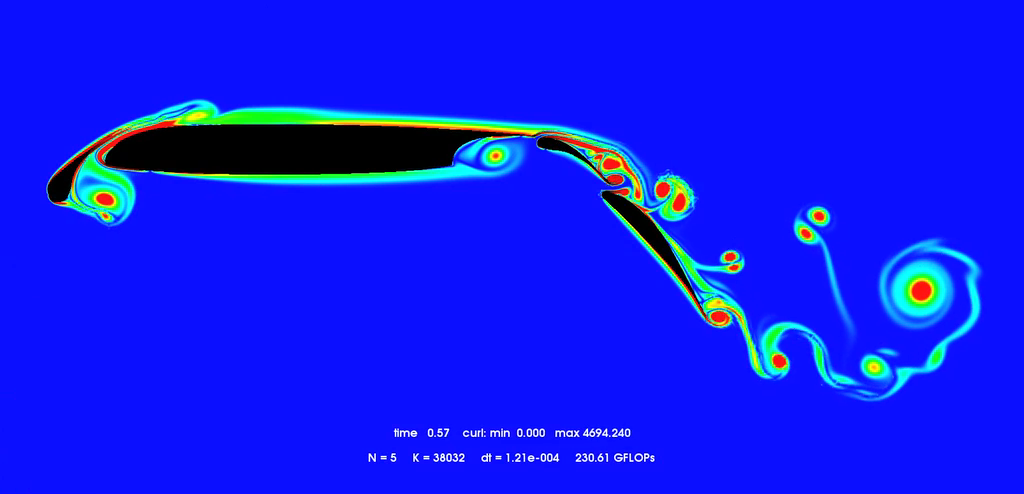
\includegraphics[width=.95\textwidth]{figs/wingflow.png}\\
%\vspace{1em}
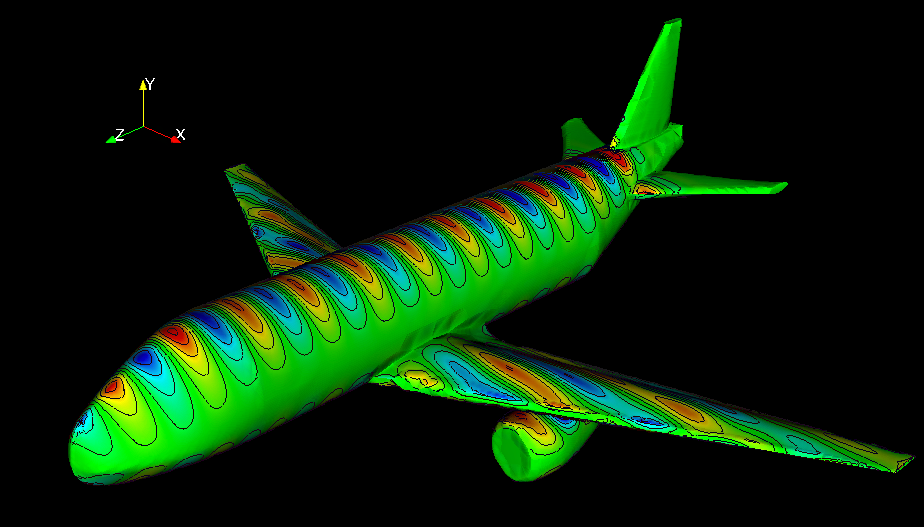
\includegraphics[width=.95\textwidth]{figs/airplane.png}
%\vspace{1em}
\caption*{\tiny Figures courtesy of T.\ Warburton.}
}
\only<2>{
\includegraphics[width=.95\textwidth]{figs/wave_N1.eps}
\caption*{\textbf{Fine} linear approximation.}
}
\only<3>{
\includegraphics[width=.95\textwidth]{figs/wave_N2.eps}
\caption*{\textbf{Coarse} quadratic approximation.}
}
\only<4-5>{
\vspace{1em}
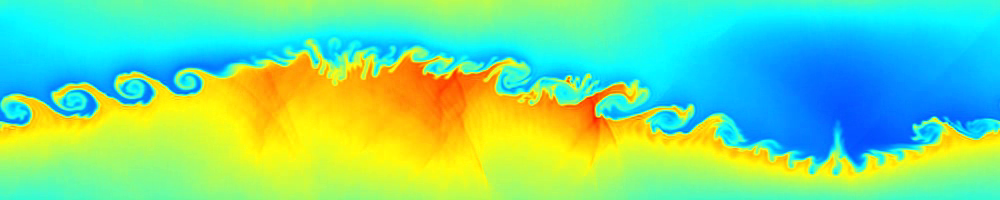
\includegraphics[width=.95\textwidth]{figs/turbulent1.png}\\
\vspace{1em}
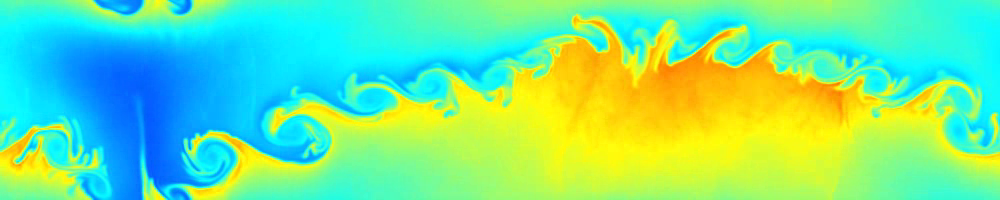
\includegraphics[width=.95\textwidth]{figs/turbulent2.png}
\caption*{\tiny Figure courtesy of Per-Olof Persson.}
}

\only<6->{
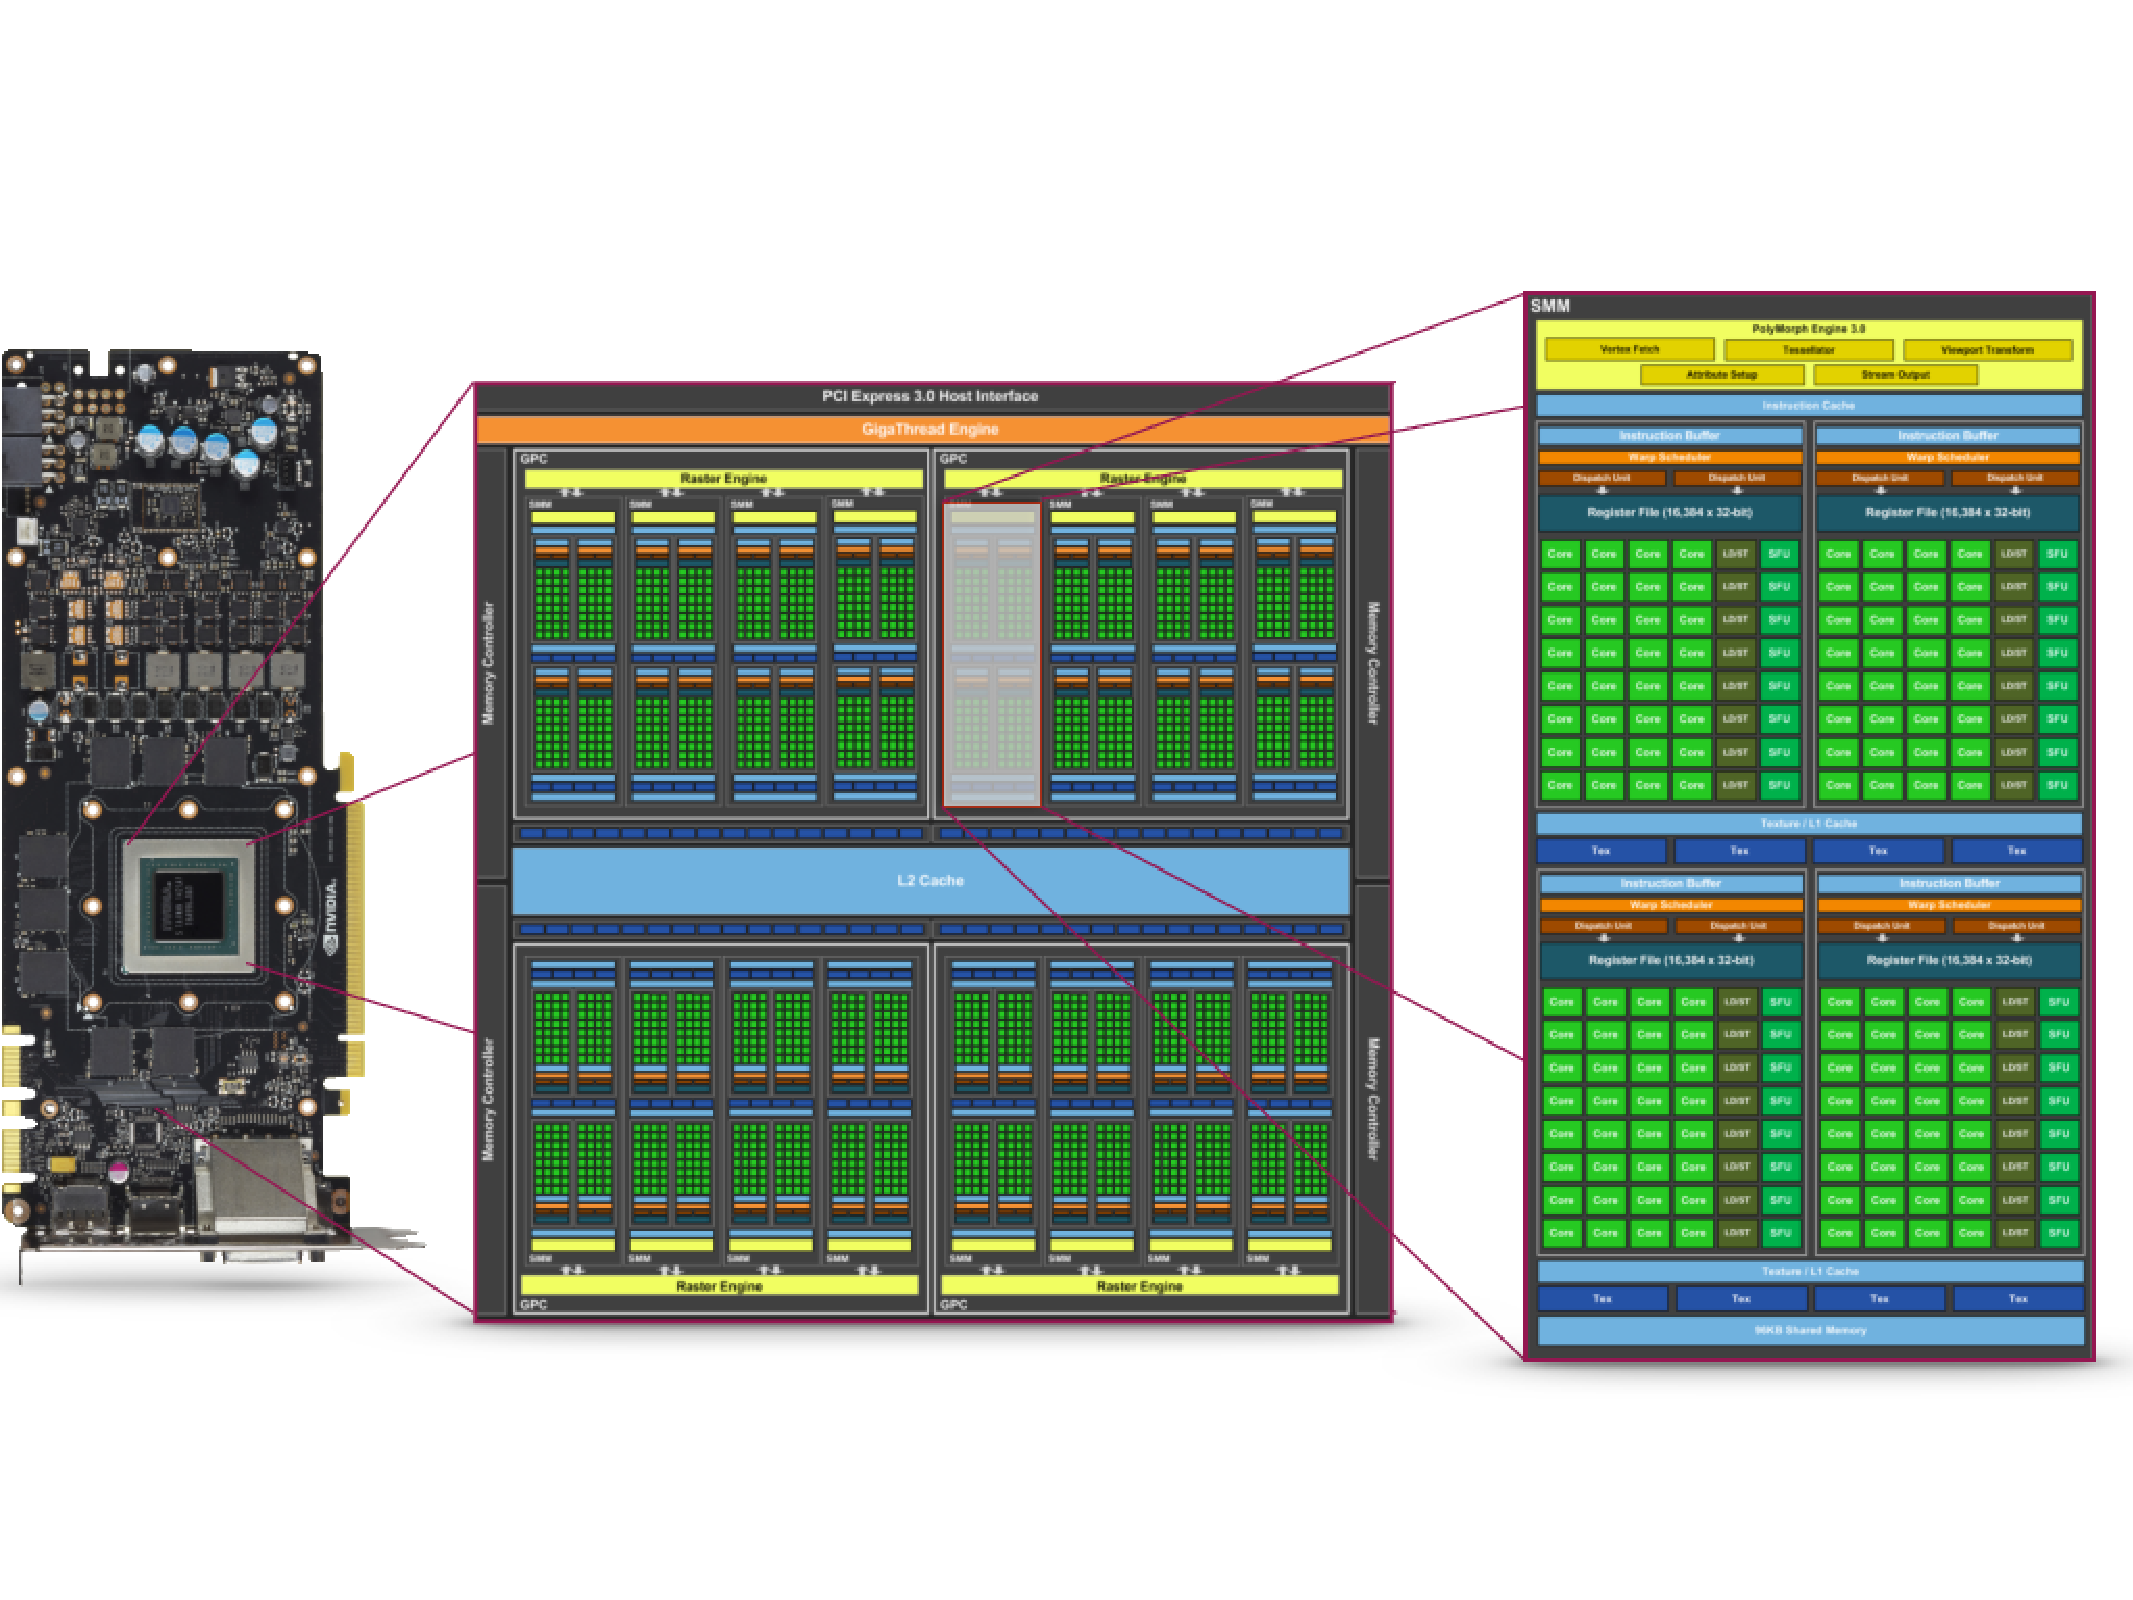
\includegraphics[width=.975\textwidth]{figs/gpu.pdf}
\caption*{A graphics processing unit (GPU).}
}
%\caption*{Image courtesy of Axel Modave.}
\end{overlayarea}
\end{figure}
\end{column}
\end{columns}
\vspace{2em}
\only<7>{
\begin{center}
\ovalbox{Goal: address inherent \note{instability} of high order methods!}
\end{center}
}
\end{overlayarea}
}

%% =================================================
\frame[noframenumbering]{
\frametitle{Talk outline}
\tableofcontents
}

\frame[noframenumbering]{
\frametitle{Talk outline}
\tableofcontents[currentsection]
}

%% =================================================


\frame{
\frametitle{High order DG methods for linear problems}% and nonlinear conservation laws}

\begin{itemize}
\item Constant \note{linear} advection on $[-1,1]$
\[
\pd{u}{t} + \pd{u}{x} = 0, \qquad u(-1) = u(1).
\]
\item 
\only<1>{
Semi-discrete form: let $\jump{u} = u^+ - u$ and $\tau \geq 0$%$\avg{u} = \frac{u^+ + u}{2}, \quad \jump{u} = u^+ - u$.
\begin{align*}
\sum_k\int_{D^k} \LRp{\pd{u}{t} + \pd{u}{x}}v + 
\int_{\partial D^k} \frac{n_x-\tau\LRb{n_x}}{2} \jump{u}v  = 0, \qquad \forall v \in V_h.
%\int_{\partial D^k} (\avg{u}-u) v n_x - \tau\frac{\LRb{n_x}}{2}\jump{u}v  = 0.% \qquad \forall v\in V_h
\end{align*}
}
%\only<2>{
%Method of lines: system of ODEs for dofs $\bm{u}$ (explicit time-stepping)
%\[
%\bm{M}_h \pd{\bm{u}}{t} = \bm{A}_h \bm{u}.
%\]
%}
\end{itemize}
\vspace{-.5em}
\begin{overlayarea}{\textwidth}{.475\textheight}
\begin{figure}
\centering
\subfloat[Central flux ($\tau = 0$)]{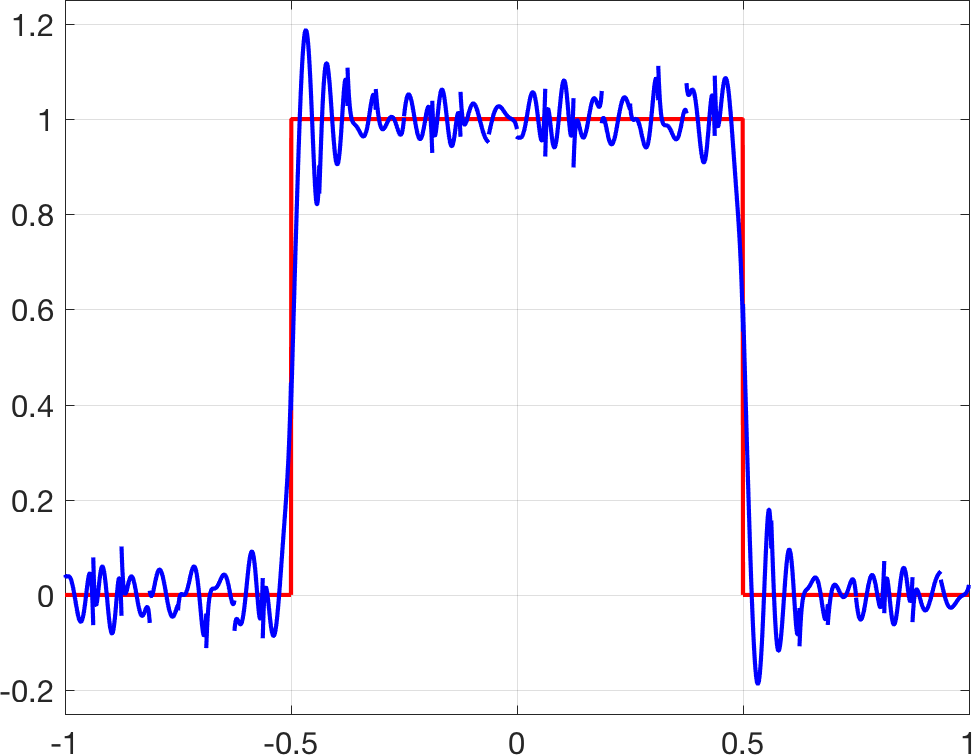
\includegraphics[width=.32\textwidth]{figs/advecCentral.png}}
\hspace{4em}
\subfloat[Upwind flux ($\tau = 1$)]{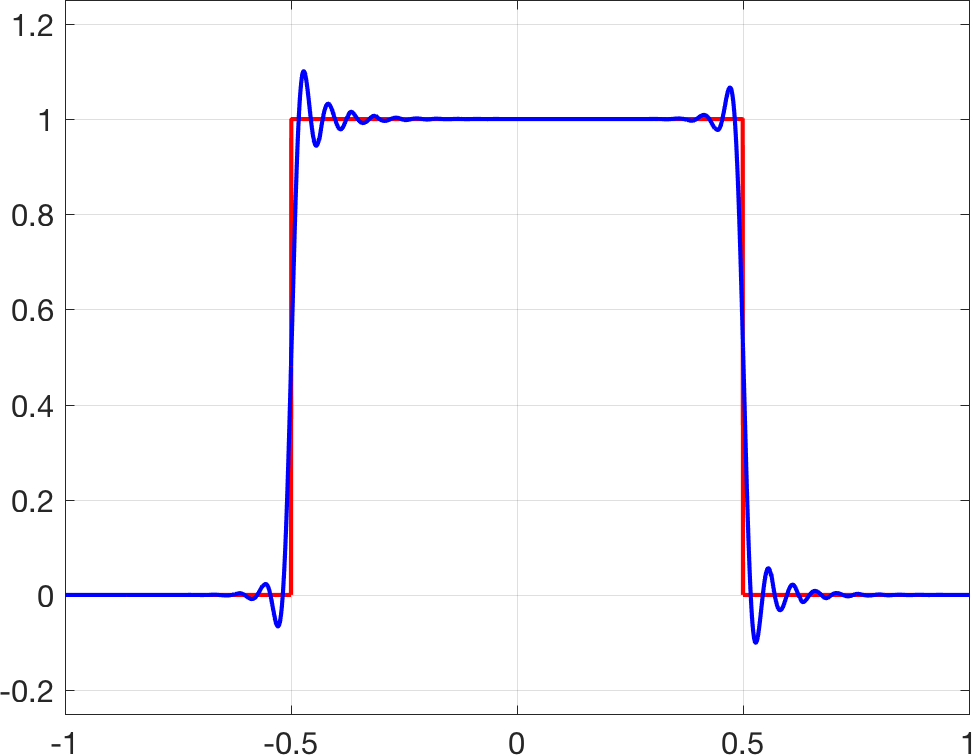
\includegraphics[width=.32\textwidth]{figs/advecUpwind.png}}
\end{figure}
\end{overlayarea}
}

%% =================================================

\frame{
\frametitle{DG energy estimates for linear advection }

\begin{itemize}
\item Let $V_h = \bigoplus_k P^N\LRp{D^k}$, define global DG derivative $D^x_h: V_h \rightarrow V_h$:
\begin{align*}
\LRp{D^x_h u,v}_{\Omega} &= \sum_{D^k} \LRp{\pd{u}{x},v}_{D^k} + \frac{1}{2}\LRa{\jump{u},v}_{\partial D^k}, \qquad v\in V_h,\\
\LRp{D^x_h u,v}_{\Omega} &= \LRa{ u,v}_{\partial \Omega} - \LRp{u, D^x_hv}_{\Omega}, \qquad \text{(integration-by-parts)}.
\end{align*}
\item Advection formulation: semi-definite penalization $s(u,v)$
\[
\LRp{\pd{u}{t} + D^x_h u,v}_{\Omega} + \underbrace{\sum_{k} \LRa{-\tau\frac{\LRb{n_x}}{2} \jump{u},v}_{\partial D^k}}_{s(u,v) \text{, pos.\ semi-def.}}.
\]
\item Energy method (periodic domains): take $v = u$, integrate by parts
\begin{align*}
\frac{1}{2}\pd{}{t} \nor{u}^2_{L^2\LRp{\Omega}} = -s(u,u) \leq 0.
\end{align*}

\end{itemize}
}

%% =================================================

\section{Nonlinear stability for conservation laws} 

\frame[noframenumbering]{
\frametitle{Talk outline}
\tableofcontents[currentsection]
}

\frame{
\frametitle{Entropy stability for nonlinear conservation laws}
\begin{itemize}
\item System of nonlinear conservation laws, convex \note{entropy} $S(\bm{u})$
\[
\pd{\bm{u}}{t} + \pd{\bm{f}(\bm{u})}{x} = 0, \qquad \bm{v} = \pd{S}{\bm{u}}.  
\]
\item \textcolor{red}{Nonlinear} entropy inequality: chain rule + entropy potential $\psi$
\begin{align*}
&\bm{v}^T\LRp{\pd{\bm{u}}{t} + \pd{\bm{f}(\bm{u})}{x}} = 0 \\
&\Longrightarrow {\pd{S(\bm{u})}{t} + \LRu{\LRp{\bm{v}^T\bm{f}(\bm{u}) - \psi(\bm{u})}}_{-1}^1 \leq 0}.
\end{align*}
\item Periodic linear advection: square entropy, $\bm{v} = \bm{u}$
\[
\int_{\Omega} \pd{S(u)}{t} \leq 0, \qquad S(u) = \frac{u^2}{2}.
\]
\end{itemize}
}

%% =================================================

\frame{
\frametitle{Discrete instability for nonlinear conservation laws}
\setcounter{subfigure}{0}

\begin{itemize}
\item How to differentiate $f({u})$?  Burgers' equation: $f(u) = u^2/2$
\[
\pd{u}{t} + \frac{1}{2}\pd{u^2}{x} = 0, \qquad u \in V_h, \quad u^2 \not\in V_h.
\]
%\[
%\pd{u}{t} + \frac{1}{2}\pd{u^2}{x} = \pd{u}{t} + u\pd{u}{x} = 0.%, \qquad 
%\]
%\item Conservation of entropy $S(u) = u^2/2$: multiply by $u$ and integrate
%\begin{align*}
%&\int_{-1}^1 u\pd{u}{t} + u^2\pd{u}{x} = \int_{-1}^1 \frac{1}{2}\pd{u^2}{t} + \frac{1}{3}\pd{u^3}{x}
%= \int_{-1}^1 \pd{S(u)}{t} + \LRu{\frac{u^3}{3}}_{-1}^1 = 0&
%%&\\
%%&\Longrightarrow \pd{}{t}\int_{-1}^1 \frac{u^2}{2} + \LRu{\frac{u^3}{3}}_{-1}^1 = 0&
%\end{align*}
\item Loss of chain rule with $L^2$ projection $P_N$ or inexact quadrature.  
\[
\LRp{\pd{u}{t} + \frac{1}{2}D^x_h P_N u^2,v}_{\Omega} = 0, \qquad \frac{1}{2}\pd{P_N u^2}{x} \neq P_N \LRp{u \pd{u}{x}}
\]
\end{itemize}
\vspace{-.75em}
%\note{Show instability of Burgers' equation using $u_0(x) = \sin(\pi x)$.}
\begin{figure}
\begin{overprint}
\centering
\foreach \id in {1,2,3,4}{%
\only<\id>{
\subfloat[$N = 7, K = 8$]{\includegraphics[width=.32\textwidth]{figs/burgersStable_\id.png}}%
\hspace{2em}%
\subfloat[$N = 7, K = 9$]{\includegraphics[width=.32\textwidth]{figs/burgersUnstable_\id.png}}
}
}
\end{overprint}

\end{figure}
}

%% =================================================

\frame{
\frametitle{Entropy stable (ES) summation-by-parts (SBP) methods}

\begin{itemize}
\item Entropy {conservation}: needs \note{mass lumping, nodal collocation}!  %$\bm{u}$
%(let $\bm{u}(x) \in \mathbb{R}^n$, $\bm{M},\bm{S},\bm{B} \rightarrow \bm{I}_n \otimes \LRp{\bm{M},\bm{S},\bm{B}}$)
\begin{align*}
&\LRp{\bm{I}_n\otimes \bm{M}}\pd{\bm{u}}{t} + \LRp{2\LRp{\bm{I}_n\otimes \bm{S}}\circ \bm{F}_S}\bm{1} = 0,& &\text{(Semi-discrete form)}&\\
&\Longrightarrow \bm{1}^T\LRp{\bm{M}\pd{S}{t} + \bm{B}\LRp{\bm{v}^T\bm{f} - \bm{\psi}}} = 0,& &\text{(Entropy conservation)}&
\end{align*}
%\item Relies on diagonal norm SBP finite differences (e.g.\ DG-SEM).
%\[
%\bm{M} = {\rm diag}(\bm{w}),
%\qquad
%\begin{array}{c}
%\bm{S} = \bm{M}\bm{D}\\
%\\
%\bm{S}  = \bm{B} - \bm{S}^T
%\end{array}, 
%\qquad 
%\bm{B} = \left(\begin{array}{cccc}-1\\&0&&\\ &&\ddots& \\ & & & 1\end{array}\right).
%\]
%\begin{overlayarea}{\textwidth}{.275\textheight}
%\only<1>{
%\[
%\underbrace{\bm{M}\pd{\bm{u}}{t} + \LRp{2\bm{S}\circ \bm{F}_S}\bm{1} = 0}_{\text{Semi-discrete form}}
%\]
%}
%\only<2>{
%\[
%\note{\underbrace{\bm{v}^T}_{\text{Test w/entropy vars}}}\LRp{\bm{M}\pd{\bm{u}}{t} + \LRp{2\bm{S} \circ \bm{F}_S}\bm{1}} = 0.
%\]
%}
%\only<3>{
%\[
%\note{\underbrace{\bm{1}^T\bm{M}\pd{S}{t}}_{
%\substack{\bm{v}^T\bm{M}\pd{\bm{u}}{t} = \bm{1}^T\bm{M}\pd{S}{\bm{u}}^T\pd{\bm{u}}{t}\\ 
%\text{Diag }\bm{M}}
%}} + \bm{v}^T\LRp{2\bm{S}\circ \bm{F}_S}\bm{1} = 0.
%\]
%}
%\only<4>{
%\[
%\bm{1}^T\bm{M}\pd{S}{t} + \bm{v}^T \bigg(\note{\underbrace{\LRp{\bm{B} + \bm{S} - \bm{S}^T}}_{\text{SBP}}} \circ \bm{F}_S\bigg)\bm{1} = 0
%\]
%}
%\only<5>{
%\[
%\bm{1}^T\bm{M}\pd{S}{t} + \note{\bm{v}^T\LRp{\bm{B} \circ \bm{F}_S}\bm{1} + \bm{v}^T\LRp{\LRp{\bm{S} - \bm{S}^T}\circ \bm{F}_S}\bm{1}} = 0
%\]
%}
%\only<6>{
%\[
%\bm{1}^T\bm{M}\pd{S}{t} + \note{\underbrace{\bm{1}^T\bm{B}\bm{v}^T\bm{f}}_{
%\substack{\bm{v}^T \LRp{\bm{B} \circ \bm{F}_S}\bm{1}\\ \text{Consistent }\bm{F}_S, \text{ diag }\bm{B}}
%}} + \bm{v}^T\LRp{\LRp{\bm{S} - \bm{S}^T}\circ \bm{F}_S}\bm{1} = 0. %\qquad \text{(Diag $\bm{B}$, $\bm{F}_S(\bm{u},\bm{u}) = \bm{f}(\bm{u})$)}
%\]
%}
%\only<7>{
%\[
%\bm{1}^T\bm{M}\pd{\bm{S}}{t} + \bm{1}^T\bm{B}\LRp{\bm{v}^T\bm{f} - \bm{\psi}} = 0.
%\]
%%\begin{center}
%$\Longrightarrow$ Discrete statement of entropy conservation!
%%\end{center}
%}
%\end{overlayarea}
\end{itemize}
\vspace{-1em}
\begin{figure}
\centering
\begingroup
\captionsetup[subfloat]{width=.275\textwidth}
\subfloat[Tensor product SBP nodes (GLL quadrature)]{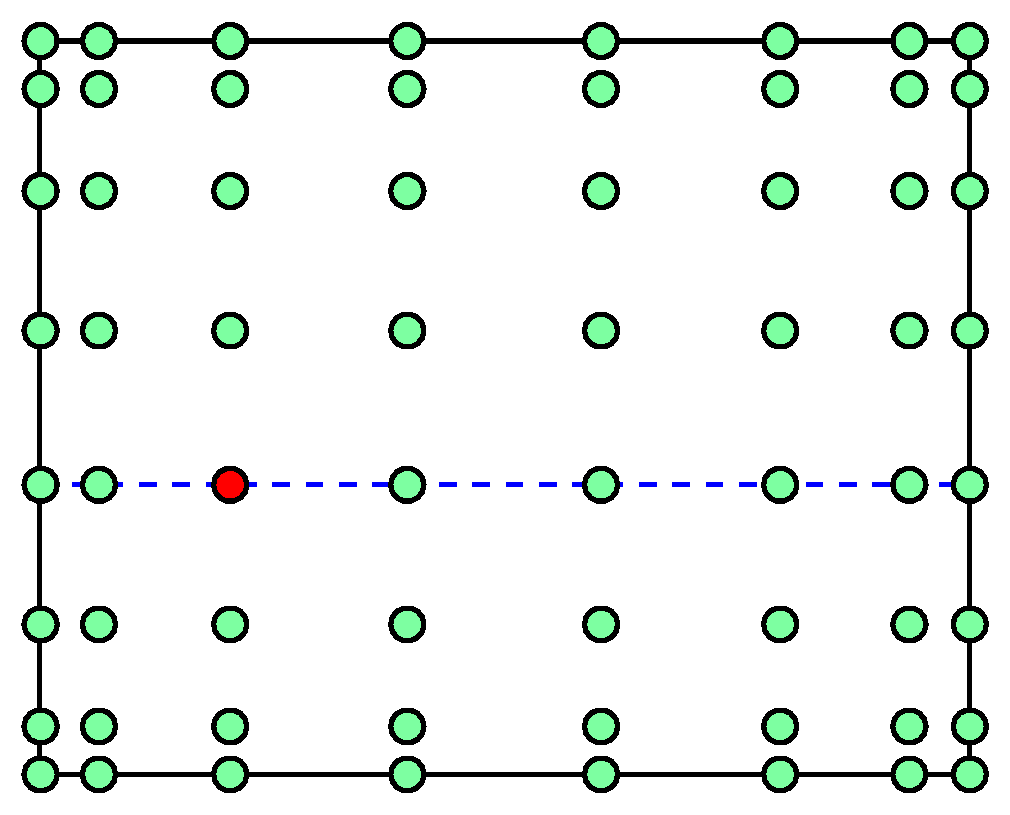
\includegraphics[width=.25\textwidth]{figs/SEM_stencil_1.pdf}}
\hspace{2.5em}
\subfloat[Diag-norm SBP nodes ($N=4$, 22 pts)]{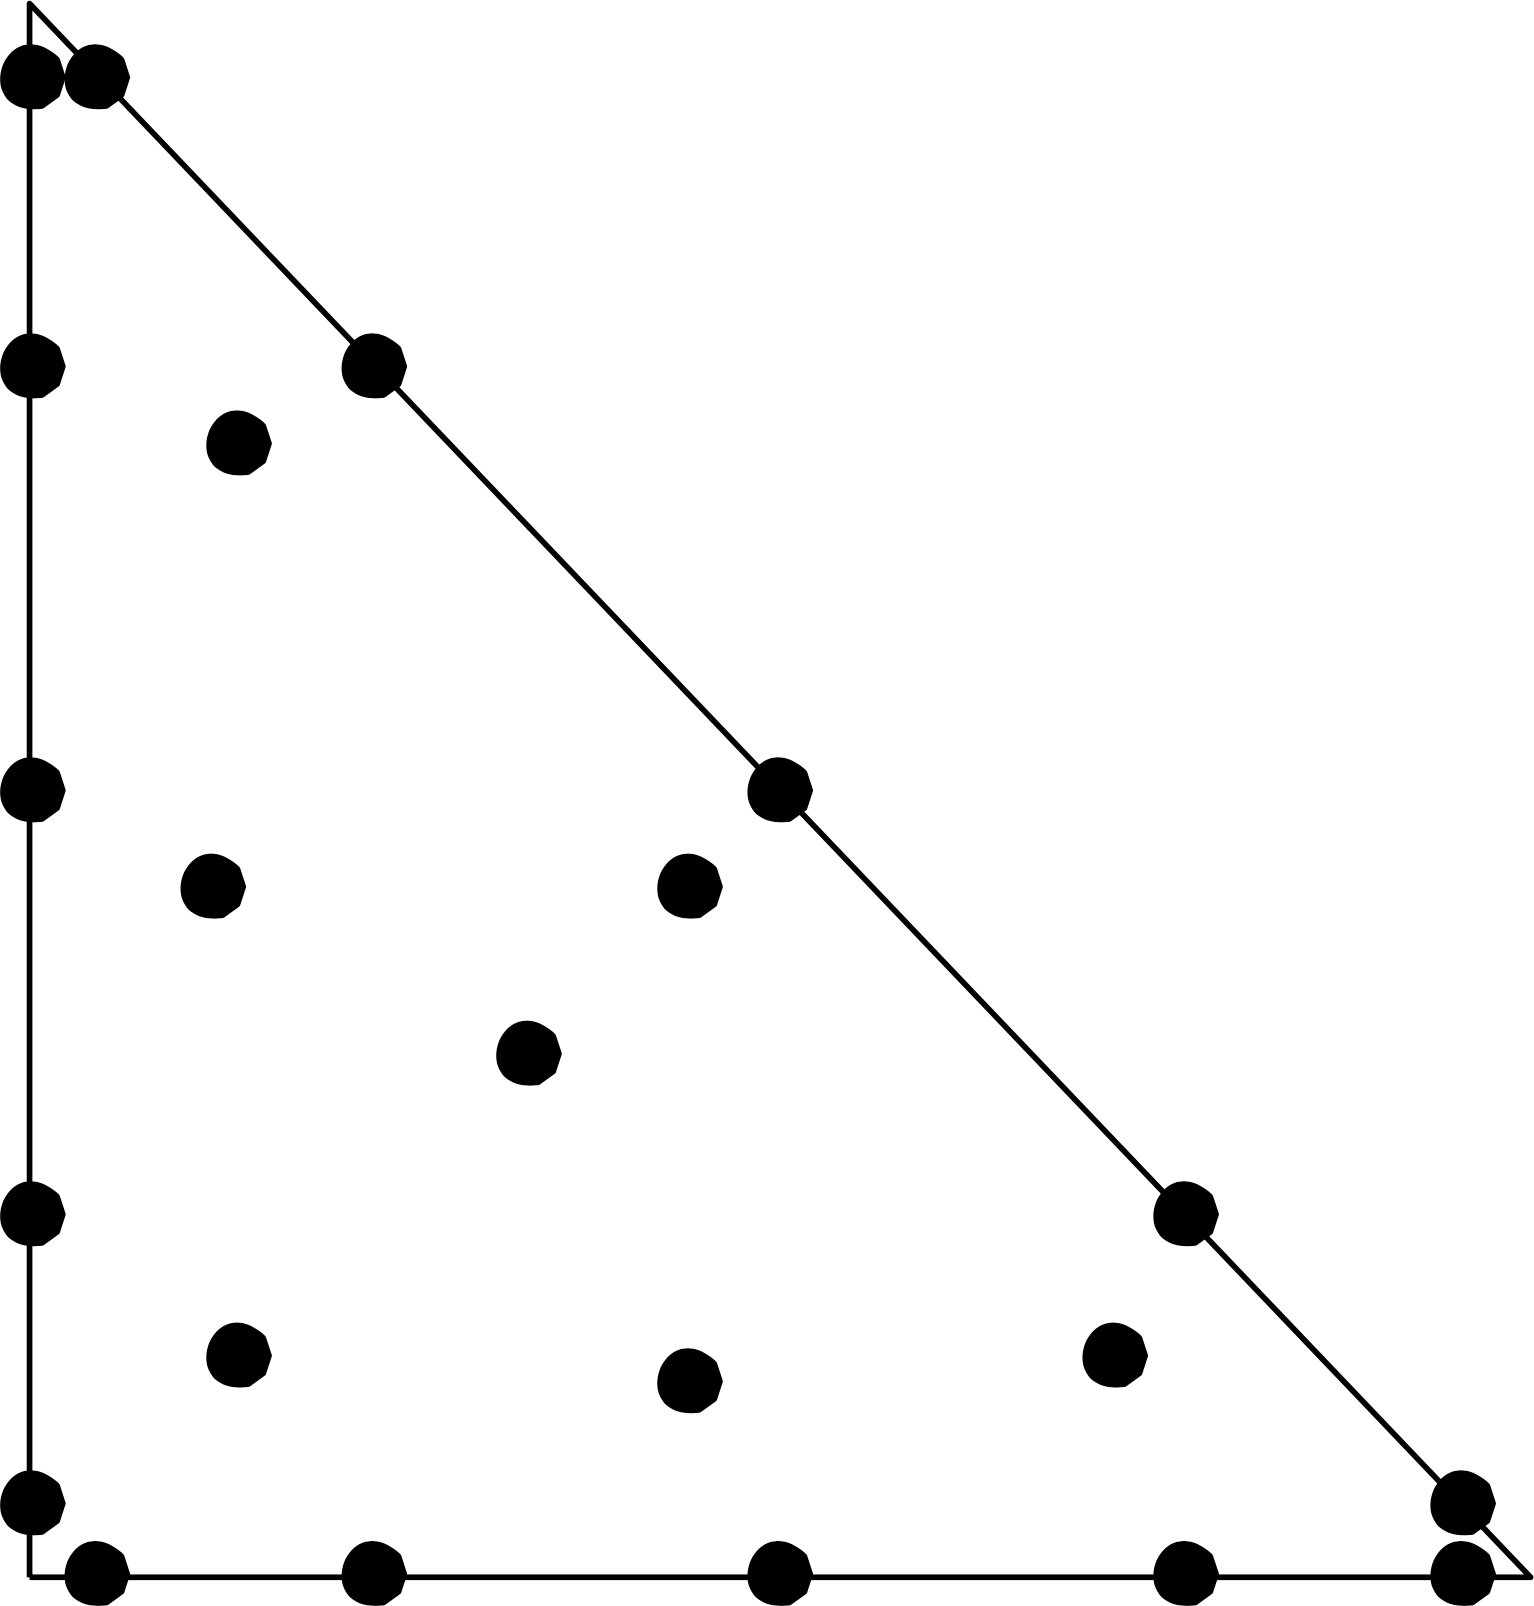
\includegraphics[height=.285\textheight]{figs/chenShuNodes.png}}
\hspace{2.5em}
\subfloat[Non-SBP nodes ($N=4$, 15 pts)]{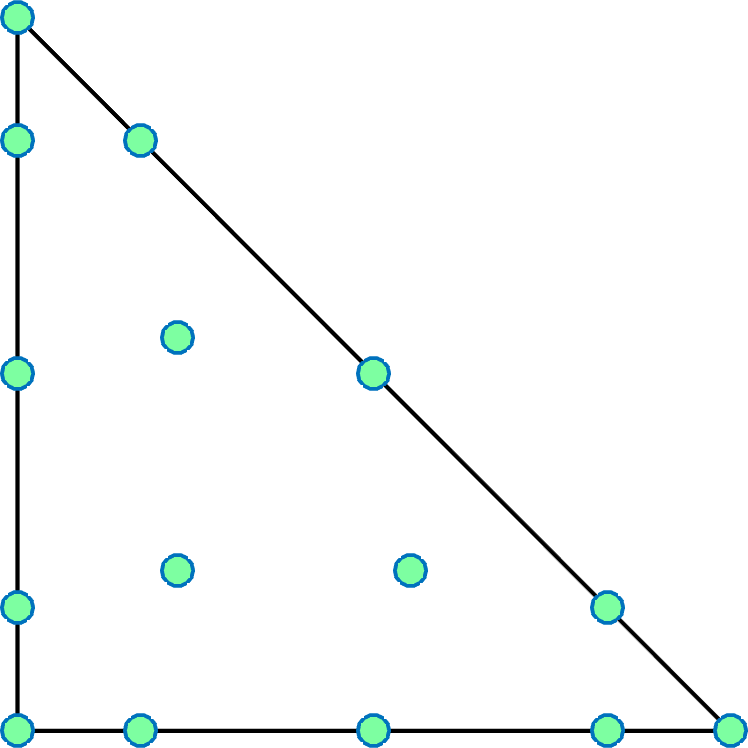
\includegraphics[height=.285\textheight]{figs/triNodesN4.png}}
\endgroup
%\caption{Dif.}
\end{figure}

\let\thefootnote\relax\footnotetext{\tiny Fisher and Carpenter (2013). \textit{High-order ES finite difference schemes for nonlinear conservation laws: Finite domains.} }
%\let\thefootnote\relax\footnotetext{\tiny Carpenter et al.\ (2014). \textit{Entropy stable spectral collocation schemes for the NS equations: discontinuous interfaces.}}
\let\thefootnote\relax\footnotetext{\tiny Gassner, Winters, and Kopriva (2016). \textit{Split form nodal DG schemes with SBP property for the comp.\ Euler equations.}}
\let\thefootnote\relax\footnotetext{\tiny Chen and Shu (2017). \textit{ES high order DG methods with suitable quadrature rules for hyperbolic conservation laws.}}

}

%% =================================================

%\frame{
%\frametitle{Challenges for summation-by-parts formulations (SBP)}
%\setcounter{subfigure}{0}
%\begin{itemize} 
%\item Construction using \note{nodal collocation} at quadrature points.  
%\item Need at least $2N-1$ accurate volume and surface quadrature! 
%\item Difficult to generalize beyond polynomial DG (splines, pyramids, etc).
%\end{itemize}
%\vspace{-.5em}
%\begin{figure}
%\centering
%\begingroup
%\captionsetup[subfloat]{width=.3\textwidth}
%\subfloat[Tensor product SBP nodes (GLL quadrature)]{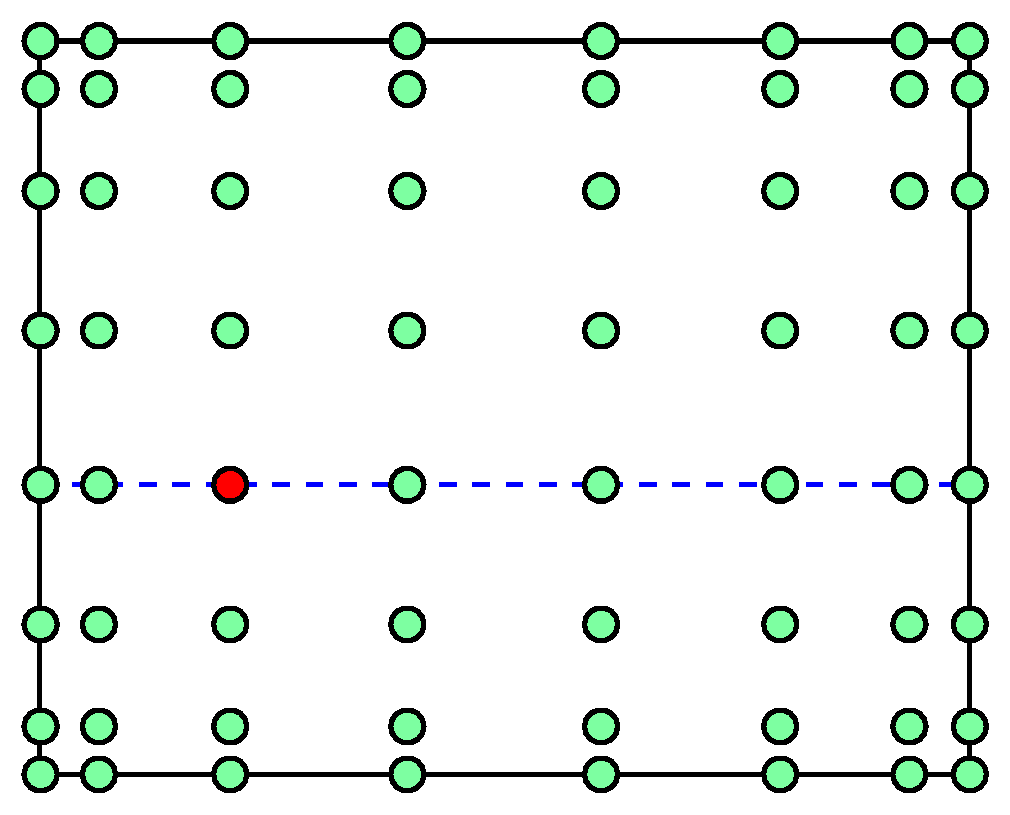
\includegraphics[width=.32\textwidth]{figs/SEM_stencil_1.pdf}}
%\hspace{1em}
%\subfloat[Interpolation nodes ($N=4$, 15 pts)]{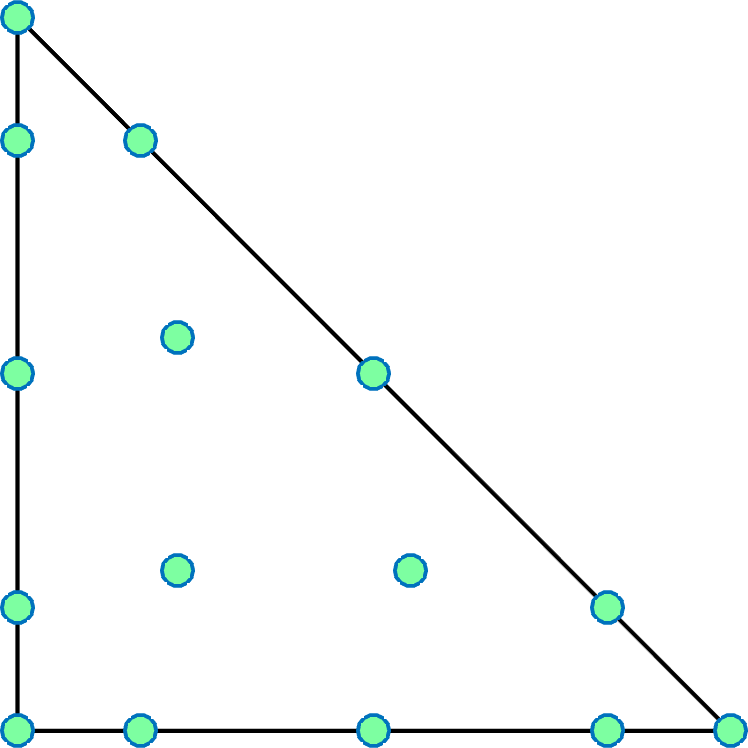
\includegraphics[width=.25\textwidth]{figs/triNodesN4.png}}
%\hspace{.5em}
%\subfloat[Diag-norm SBP nodes ($N=4$, 22 pts)]{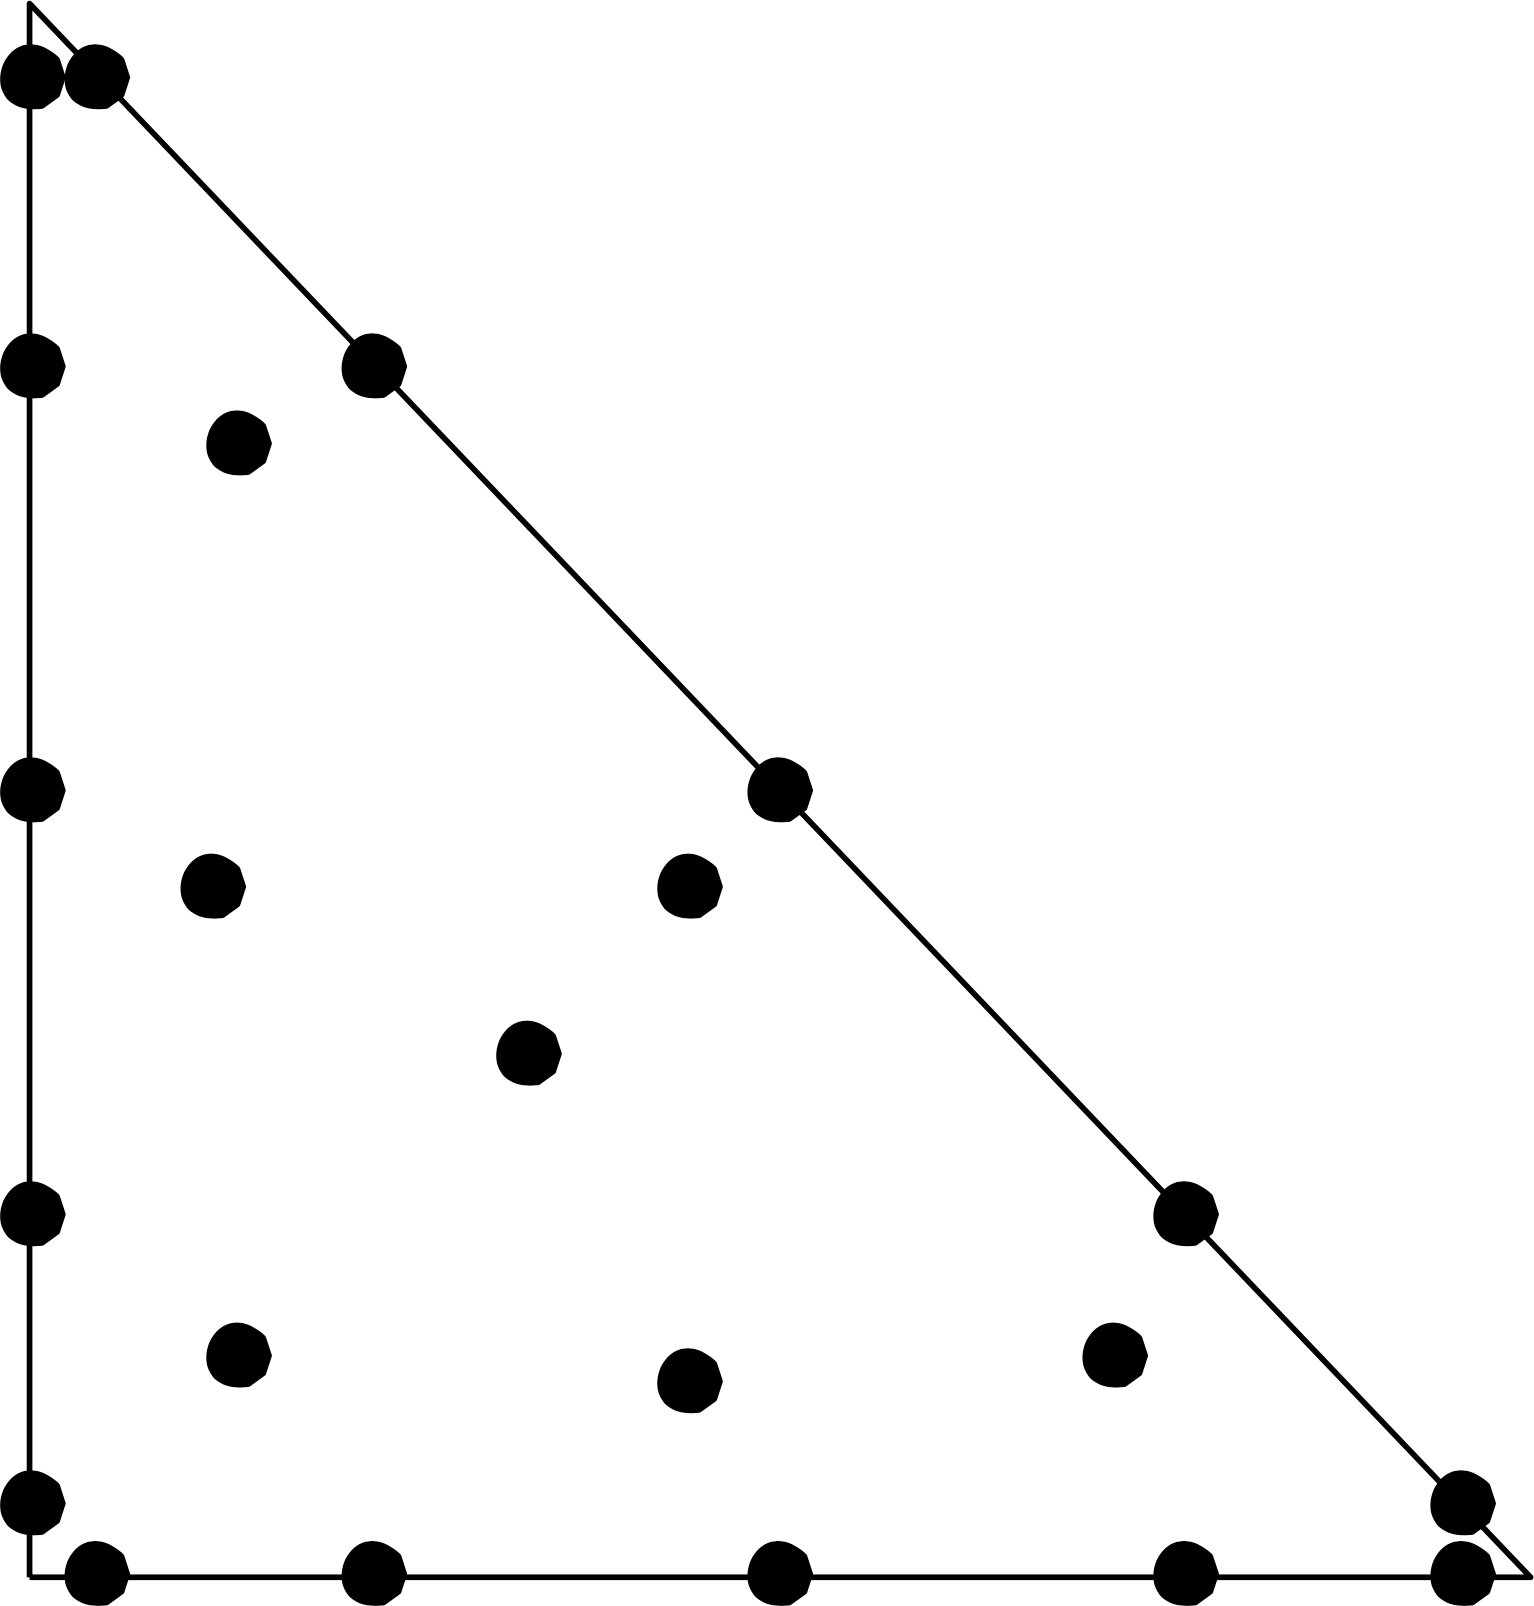
\includegraphics[width=.25\textwidth]{figs/chenShuNodes.png}}
%\endgroup
%%\caption{Dif.}
%\end{figure}
%
%\let\thefootnote\relax\footnotetext{\tiny Chen and Shu (2017). \textit{ES high order DG methods with suitable quadrature rules for hyperbolic conservation laws.}}
%\let\thefootnote\relax\footnotetext{\tiny Chan and Evans (2017). \textit{Multi-patch DG spline finite element methods for time-domain wave propagation}.}
%}


%% =================================================

\section{Continuous entropy stable formulations} 

\frame[noframenumbering]{
\frametitle{Talk outline}
\tableofcontents[currentsection]
}

\frame{
\frametitle{Burgers' equation: energy stable formulations}
\setcounter{subfigure}{0}
\begin{itemize}
\item Split formulation (replace $\pd{}{x}$ with some $D^x_h$ + stabilization for DG).
\begin{align*}
&\pd{u}{t} + \frac{1}{3}\LRp{\pd{u^2}{x} + {u\pd{u}{x}}} \Longrightarrow \pd{u}{t} + \frac{1}{3}\LRp{D^x_h P_N u^2 + P_N\LRp{uD^x_h u}} = 0\\
&\Longrightarrow \frac{1}{2}\pd{}{t}\nor{u}^2_{L^2(\Omega)} + \frac{1}{3}
%\LRp{\LRp{\pd{P_N u^2}{x},u} - \LRp{u,\pd{P_N u^2}{x}} + 
{\LRa{u^2,u}_{\partial \Omega}}  = 0.
\end{align*}
\end{itemize}
%\vspace{-.25em}
\begin{figure}
\begin{overlayarea}{\textwidth}{.5\textheight}
%\begin{overprint}
\centering
\foreach \id in {1,2,3,4,5,6,7,8}{%
\only<\id>{
\subfloat[$\tau = 0$]{\includegraphics[width=.35\textwidth]{figs/burgersStableEC_\id.png}}\hspace{2em}%
\subfloat[$\tau = 1$]{\includegraphics[width=.35\textwidth]{figs/burgersStableLF_\id.png}}
}% \only
}% for
\only<9>{
\subfloat[Energy conservative ($\tau = 0$)]{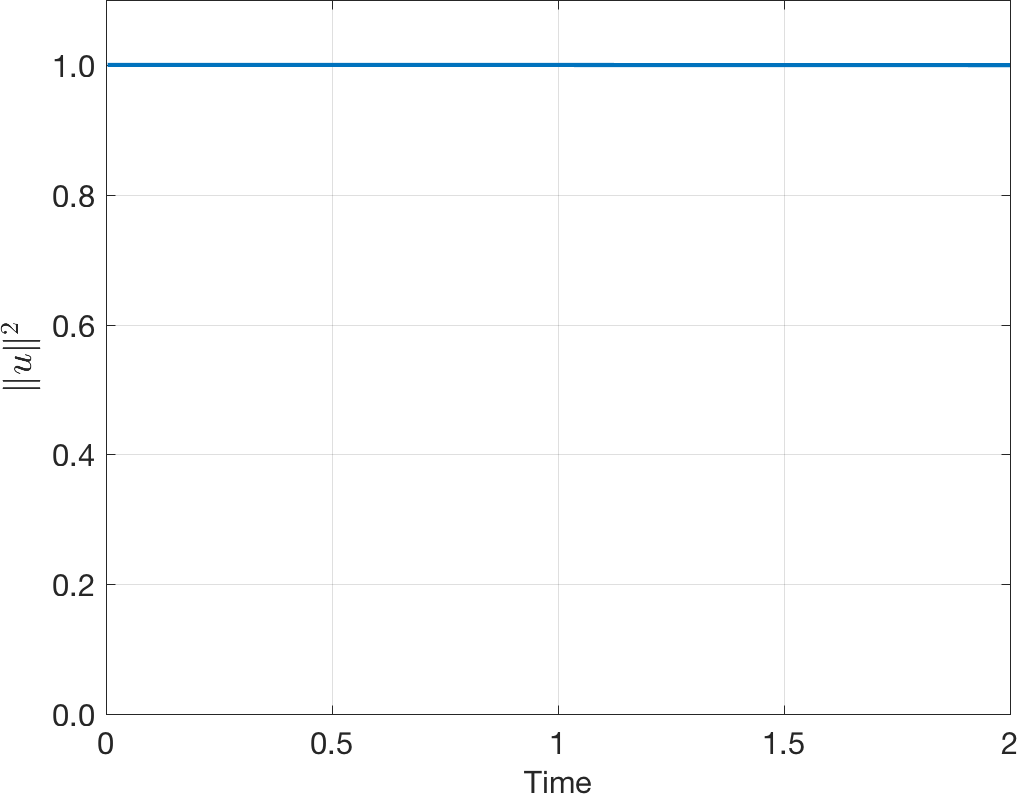
\includegraphics[width=.425\textwidth]{figs/burgersSplitEnergyEC.png}}\hspace{1em}%
\subfloat[Energy stable ($\tau = 1$)]{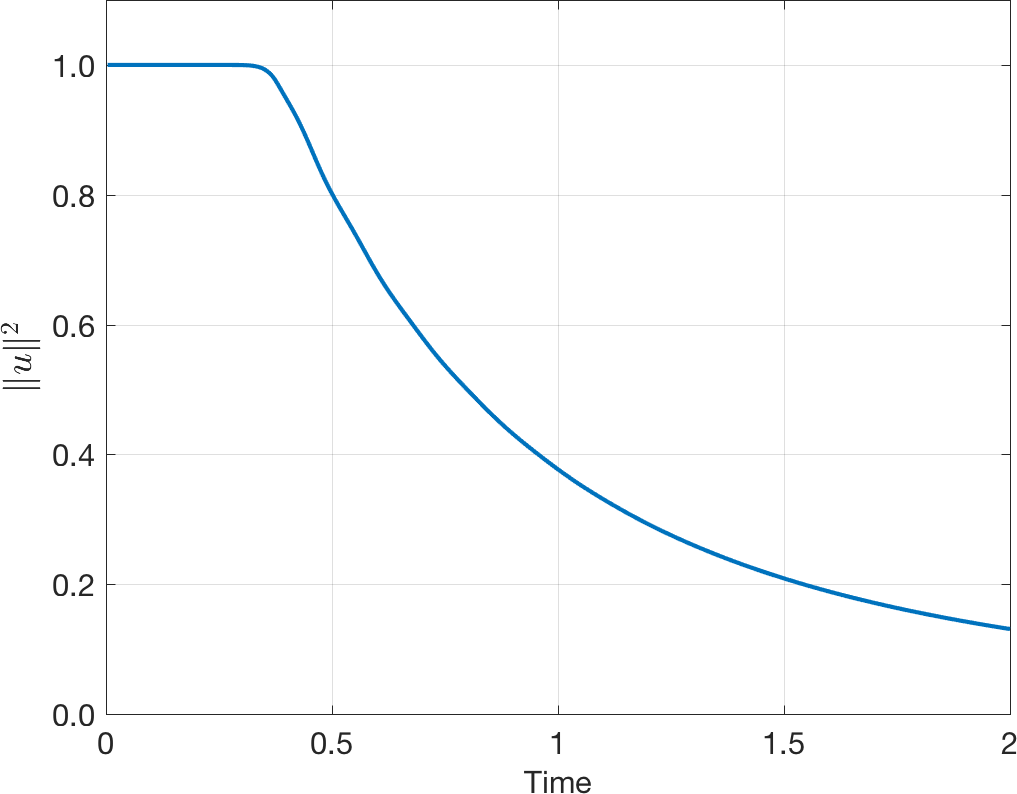
\includegraphics[width=.425\textwidth]{figs/burgersSplitEnergyLF.png}}
}
%\end{overprint}
\end{overlayarea}
\end{figure}
}
%% =================================================


\frame{
\frametitle{Flux differencing: split formulations and beyond}

\begin{itemize}
\item<1-> Tadmor's entropy conservative finite volume flux
\begin{align*}
\bm{f}_S(\bm{u},\bm{u}) &= \bm{f}(\bm{u}), \qquad \text{(consistency)} \\
\bm{f}_S(\bm{u},\bm{v}) &= \bm{f}_S(\bm{v},\bm{u}),\qquad \text{(symmetry)} \\
\LRp{\bm{v}_L - \bm{v}_R}^T \bm{f}\LRp{\bm{u}_L,\bm{u}_R} &= \psi_L - \psi_R, \qquad \text{(conservation)}.
\end{align*}
\item<2-> Easy example: Burgers' equation, let $u_L = u(x), u_R = u(y)$
\begin{align*}
&f_S(u_L,u_R) = \frac{1}{6}\LRp{u(x)^2 + u(x)u(y) + u(y)^2},\\ %\qquad \bm{v} = u, \qquad \psi = \frac{u^3}{3}\\
\pd{{f}({u})}{x} &\Longrightarrow \note{\LRu{2\pd{f_S\LRp{u_x,u_y}}{x}}_{y=x}} = \frac{1}{3}\pd{u^2}{x} + \frac{1}{3}u\pd{u}{x} + \frac{1}{3}u^2\cancel{ \pd{1}{x}}.
\end{align*}
\item<3> Harder example: compressible Euler (entropy conservative mass flux)
\[
f^{\rho}_S(\bm{u}_L,\bm{u}_R) = \avg{\rho}^{\log} \avg{u}, \qquad \avg{u}^{\log} = \frac{u_L - u_R}{\log{u_L}- \log{u_R}}.
\]
\end{itemize}

\let\thefootnote\relax\footnotetext{\tiny Chandrashekar (2013). \textit{Kinetic energy preserving and entropy stable FV schemes for compressible Euler and NS equations.}}
}

%% =================================================

\frame{
\frametitle{Discrete entropy conservation: a continuous formulation}
\vspace{-1em}
\begin{overlayarea}{\textwidth}{.9\textheight}
\begin{theorem}[Chan 2017]
Let $\bm{u}_{x} =  \bm{u}\LRp{(P_N \bm{v})(x)}, \bm{u}_{y} = \bm{u}\LRp{(P_N \bm{v})(y)}$, and let $\bm{u}$ solve
\[
\LRp{\pd{\bm{u}}{t} + \left.\LRp{2 D^x_h \bm{f}_S(\bm{u}_x,\bm{u}_y)}\right|_{y=x},\bm{w}}_{\Omega} = 0, \qquad \forall \bm{w}\in V_h.
\]
Then $\bm{u}$ satisfies $\int_{\Omega} \pd{S(\bm{u})}{t} + \int_{\partial \Omega} P_N\bm{v}^T\bm{f}(\bm{u}_x) - \psi(\bm{u}_x) = 0.$%a quadrature-based conservation of entropy.
%\[
%\int_{\Omega} \pd{S}{t} + \int_{\partial \Omega} \bm{v}^T\bm{f}(\bm{u}) - \psi(\bm{u}) = 0.
%\]
\end{theorem} 
\only<2-4>{
\begin{proofsketch}
\only<2>{
Step 1 (time term): take $\bm{w} = P_N \bm{v}(\bm{u})$.  For method of lines, $\pd{\bm{u}}{t} \in V_h$.
\[
\LRp{\pd{\bm{u}}{t},P_N\bm{v}}_{\Omega} = \LRp{\pd{\bm{u}}{t},\bm{v}}_{\Omega} = \LRp{\pd{S}{\bm{u}}\pd{\bm{u}}{t},1}_{\Omega} = \LRp{\pd{S(\bm{u})}{t},1}_{\Omega}.
\]
}

\only<3>{
Step 2 (spatial term): integrate by parts.  
\vspace{-.5em}
\begin{align*}
&\LRp{\LRu{\LRp{D^x_h \bm{f}_S(\bm{u}_x,\bm{u}_y)}}_{y=x},P_N\bm{v}}_{\Omega}\\
&+ \LRa{\bm{f}_S\LRp{\bm{u}_x,\bm{u}_x}, (P_N \bm{v})\bm{n}_x }_{\partial \Omega} - \LRp{\LRu{D^x_h \LRp{\bm{f}_S(\bm{u}_x,\bm{u}_y)\LRp{P_N\bm{v}}(x)}}_{y=x},1}_{\Omega}.
\end{align*}
}

%\only<3>{
%Step 2 (spatial term): gather volume terms
%\vspace{-.5em}
%\begin{align*}
%&\LRp{\LRu{\LRp{D^x_h \bm{f}_S(\bm{u}_x,\bm{u}_y)\LRp{P_N\bm{v}}(y)}}_{y=x},1}_{\Omega} \\
%&- \LRp{\LRu{D^x_h \LRp{\bm{f}_S(\bm{u}_x,\bm{u}_y)\LRp{P_N\bm{v}}(x)}}_{y=x},1}_{\Omega}.
%\end{align*}
%}

\only<4>{
Step 2 (spatial term):  gather volume terms, use conservation and IBP.
\vspace{-.5em}
\begin{align*}
&\LRp{\LRu{{D^x_h \LRp{
\note{
\bm{f}_S(\bm{u}_x,\bm{u}_y)\LRp{\LRp{P_N\bm{v}}(x)-\LRp{P_N\bm{v}}(y)}
}
}}}_{y=x},1}_{\Omega}\\
&=  \LRp{\LRu{{D^x_h \LRp{\psi(\bm{u}_x)-\psi(\bm{u}_y)}}}_{y=x},1}_{\Omega} = \LRa{\psi(\bm{u}_x),1\bm{n}_x}_{\partial \Omega}.
\end{align*}
}
%\only<4>{
%Step 2 (spatial term): gather volume terms
%\vspace{-.5em}
%\begin{align*}
%\LRp{\LRu{\LRp{D^x_h \bm{f}_S(\bm{u}_x,\bm{u}_y)}\LRp{P_N\bm{v}}(y)}_{y=x},1}_{\Omega} + \LRp{\LRu{D^x_h \LRp{\bm{f}_S(\bm{u}_x,\bm{u}_y)\LRp{P_N\bm{v}}(x)}}_{y=x},1}_{\Omega}.
%\end{align*}
%}
\end{proofsketch}
}
%\begin{itemize}
%\item \note{blah: finish this!}  Integrate by parts
%\item Use symmetry of $\bm{f}_S$ and conservation.
%\item Use consistency for the boundary integral.
%\end{itemize}

\only<5>{
%\vspace{-.25em}
\begin{itemize}
\item Difficulty: $\bm{u}\in V_h$, but $\bm{v}(\bm{u}) \not\in V_h$! 
% Recover entropy conservation by testing with \note{projected} entropy variables.  
Need $\bm{u} = \bm{u}\LRp{P_N \bm{v}}$ for
\[
\LRp{P_N\bm{v}_L - P_N\bm{v}_R}^T \bm{f}\LRp{\bm{u}_L,\bm{u}_R} = \psi_L - \psi_R.
\]
%\item \note{Diag $y=x$ formulation, $\bm{u}_x = \bm{u}_{\bm{v}}(x), \bm{u}_y = \bm{u}_{\bm{v}}(y)$}
\item Proof requires only (inexact) quadrature-based $L^2$ projection + IBP.  
\item Jump stabilization $s(u,v)$ gives entropy \note{inequality}. 
\end{itemize}
}
\end{overlayarea}

\let\thefootnote\relax\footnotetext{\tiny Chan (2017). \textit{On discretely entropy conservative and entropy stable discontinuous Galerkin methods.}}

%\let\thefootnote\relax\footnotetext{\tiny Chandrashekar (2013). \textit{Kinetic energy preserving and entropy stable FV schemes for compressible Euler and NS equations.}}
}

%% =================================================
%\begin{align*}
%f^1_S(\bm{u}_L,\bm{u}_R) &= \avg{\rho}^{\log} \avg{u}\\
%f^2_S(\bm{u}_L,\bm{u}_R) &= \frac{\avg{\rho}}{2\avg{\beta}} + \avg{u}f^1_S\\
%f^3_S(\bm{u}_L,\bm{u}_R) &= f^1_S\LRp{\frac{1}{2(\gamma-1)\avg{\beta}^{\log}} - \frac{1}{2}\avg{u^2}} + \avg{u}f^2_S,
%\end{align*}
%\[
%\avg{u}^{\log} = \frac{u_L - u_R}{\log{u_L}- \log{u_R}}, \qquad \beta = \frac{\rho}{2p}.
%\]
%\item Chandreshekar's entropy conservative and KEP flux.  


\frame{
\frametitle{Entropy stable high order DG: implementation}

\begin{itemize}
\item Efficient reformulation (Hadamard product: low-memory evaluation)
\begin{align*}
&P_N \LRp{\LRu{\pd{P_N \bm{f}_S(\bm{u}_x,\bm{u}_y)}{x}}_{y=x}} \\
&= \bm{P}_q {\rm diag}\LRp{\bm{V}_q\bm{D}\bm{P}_q \bm{F}_S} =  \bm{P}_q \LRp{\LRp{\bm{V}_q\bm{D}\bm{P}_q \circ \bm{F}_S}\bm{1}}.\\
\end{align*}
\vspace{-2em}
\item Explicit time-stepping right hand side evaluation:
\begin{enumerate}
\item Compute $P_N\LRp{\bm{v}(\bm{u})}$.
\item Evaluate $\bm{u} = \bm{u}(P_N\LRp{\bm{v}(\bm{u})})$ at volume, face quadratures.
\item Compute $\bm{RHS}(\bm{u}) = 2\LRp{\bm{D}_h \circ \bm{F}_S\LRp{\bm{u}_x,\bm{u}_y}}\bm{1}$
\end{enumerate}
\vspace{1.5em}
\item Simplifications for diag-norm SBP (nodal collocation): avoid computing projections, combine volume + surface operations.
\end{itemize}


%\begin{algorithm}[H]
%\begin{algorithmic}[1]
%\FOR{timestep $i$}
%\STATE Compute $P_N\LRp{\bm{v}(\bm{u})}$.
%\STATE Evaluate $\bm{u} = \bm{u}(P_N\LRp{\bm{v}(\bm{u})})$ at volume, face quadratures.
%\STATE (Optional) postprocess solution (positivity limiting, filtering, etc).  
%\STATE Compute $\bm{RHS}(\bm{u}) =\LRp{\bm{D}_h \circ \bm{F}_S\LRp{\bm{u}_x,\bm{u}_y}}\bm{1}$
%\STATE Update solution $\bm{u}^{k+1} = \bm{u}^k + \Delta t \bm{RHS}(\bm{u})$.
%\ENDFOR
%\end{algorithmic}
%\caption{Implementation}
%\label{alg:seq}
%\end{algorithm}

}

%% =================================================

\section{Numerical experiments, higher dimensions, curved meshes}

\frame[noframenumbering]{
\frametitle{Talk outline}
\tableofcontents[currentsection]
}

\frame{
\frametitle{Numerical experiments: compressible Euler equations}

\begin{itemize}
\item Entropy conservative (EC) and Lax-Friedrichs (LF) fluxes.  
\item No additional stabilization, filtering, or limiting.
\item $L^2$ rates: odd/even decoupling for EC, $O(h^{N+1})$ for LF.
\end{itemize} 
\vspace{-1em}
\begin{figure}
\centering
\subfloat[Entropy conservative flux]{
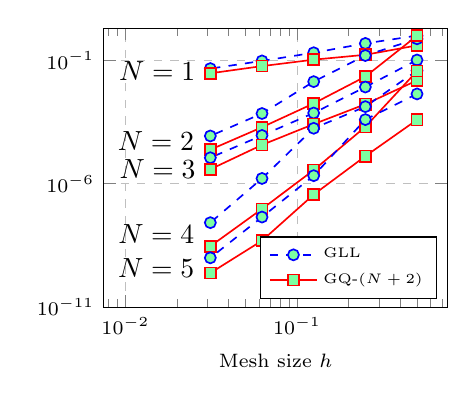
\begin{tikzpicture}
\begin{loglogaxis}[
    width=.49\textwidth,
    xlabel={Mesh size $h$},
%    ylabel={$L^2$ errors}, 
    xmin=.0075, xmax=.75,
    ymin=1e-11, ymax=2,
    legend pos=south east, legend cell align=left, legend style={font=\tiny},	
    xmajorgrids=true, ymajorgrids=true, grid style=dashed,
    legend entries={GLL,GQ-$(N+2)$}    
]
\pgfplotsset{
cycle list={{blue, dashed, mark=*}, {red, mark=square*}}
}
%\addlegendimage{no markers,blue}
%\addlegendimage{no markers,red}

\addplot+[semithick, mark options={solid, fill=markercolor}]
% N = 1, tau = 0.000000 =======================
coordinates{(0.5,1)(0.25,0.485059)(0.125,0.203599)(0.0625,0.0947163)(0.03125,0.0463705)};
\addplot+[semithick, mark options={solid, fill=markercolor}]
%N = 1, tau = 0.000000 =======================
coordinates{(0.5,0.402314)(0.25,0.167917)(0.125,0.106574)(0.0625,0.058359)(0.03125,0.0298728)}
[yshift=1pt] node[left, pos=1.025, color=black] {$N = 1$};


\addplot+[semithick, mark options={solid, fill=markercolor}]
% N = 2, tau = 0.000000 =======================
coordinates{(0.5,0.746606)(0.25,0.156701)(0.125,0.0137392)(0.0625,0.000701926)(0.03125,8.64531e-05)};
\addplot+[semithick, mark options={solid, fill=markercolor}]
%N = 2, tau = 0.000000 =======================
coordinates{(0.5,0.993771)(0.25,0.0219437)(0.125,0.00180028)(0.0625,0.000194939)(0.03125,2.4045e-05)}
[yshift=4pt] node[left, pos=1.025, color=black] {$N = 2$};


\addplot+[semithick, mark options={solid, fill=markercolor}]
% N = 3, tau = 0.000000 =======================
coordinates{(0.5,0.103299)(0.25,0.00829887)(0.125,0.00073573)(0.0625,9.05975e-05)(0.03125,1.13596e-05)};
\addplot+[semithick, mark options={solid, fill=markercolor}]
%N = 3, tau = 0.000000 =======================
coordinates{(0.5,0.0154054)(0.25,0.00167426)(0.125,0.000260859)(0.0625,3.76182e-05)(0.03125,3.86238e-06)}
[yshift=1pt] node[left, pos=1.025, color=black] {$N = 3$};

\addplot+[semithick, mark options={solid, fill=markercolor}]
% N = 4, tau = 0.000000 =======================
coordinates{(0.5,0.0385542)(0.25,0.00133048)(0.125,0.000176663)(0.0625,1.64135e-06)(0.03125,2.66024e-08)};
\addplot+[semithick, mark options={solid, fill=markercolor}]
%N = 4, tau = 0.000000 =======================
coordinates{(0.5,0.0367592)(0.25,0.000202817)(0.125,3.57758e-06)(0.0625,9.58294e-08)(0.03125,2.94985e-09)}[yshift=6pt] node[left, pos=1.025, color=black] {$N = 4$};

\addplot+[semithick, mark options={solid, fill=markercolor}]
% N = 5, tau = 0.000000 =======================
coordinates{(0.5,0.00436131)(0.25,0.00039846)(0.125,2.1282e-06)(0.0625,4.49046e-08)(0.03125,9.99912e-10)};
\addplot+[semithick, mark options={solid, fill=markercolor}]
%N = 5, tau = 0.000000 =======================
coordinates{(0.5,0.000390565)(0.25,1.31188e-05)(0.125,3.6544e-07)(0.0625,4.95271e-09)(0.03125,2.42763e-10)}
[yshift=3pt] node[left, pos=1.025, color=black] {$N = 5$};

%\legend{$N=1$,$N=2$,$N=3$,$N=4$,$N=5$}
\end{loglogaxis}
\end{tikzpicture}
}
\subfloat[With Lax-Friedrichs penalization]{
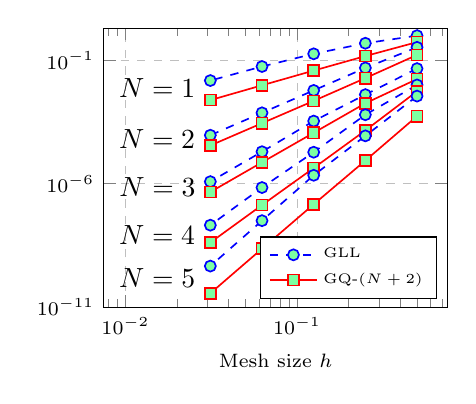
\begin{tikzpicture}
\begin{loglogaxis}[
    width=.49\textwidth,
    xlabel={Mesh size $h$},  %ylabel={$L^2$ errors}, 
    xmin=.0075, xmax=.75,
    ymin=1e-11, ymax=2,
    legend pos=south east, legend cell align=left, legend style={font=\tiny},	
    xmajorgrids=true, ymajorgrids=true, grid style=dashed,
    legend entries={GLL,GQ-$(N+2)$}
] 
\pgfplotsset{
cycle list={{blue, dashed, mark=*}, {red, mark=square*}}
}
%\pgfplotsset{cycle list={{blue, dashed, mark=*}, {red, mark=square*}}}

\addplot+[semithick, mark options={solid, fill=markercolor}]
% N = 1, tau = 0.500000 =======================
coordinates{(0.5,1)(0.25,0.4932)(0.125,0.183839)(0.0625,0.0562398)(0.03125,0.0151873)};
\addplot+[semithick, mark options={solid, fill=markercolor}]
%N = 1, tau = 0.500000 =======================
coordinates{(0.5,0.547558)(0.25,0.148981)(0.125,0.0384647)(0.0625,0.00974763)(0.03125,0.00244539)}
[yshift=5pt] node[left, pos=1.025, color=black] {$N = 1$};

\addplot+[semithick, mark options={solid, fill=markercolor}]	
% N = 2, tau = 0.500000 =======================
coordinates{(0.5,0.336817)(0.25,0.04941)(0.125,0.00605428)(0.0625,0.000748842)(0.03125,9.25456e-05)};
\addplot+[semithick, mark options={solid, fill=markercolor}]
%N = 2, tau = 0.500000 =======================
coordinates{(0.5,0.165807)(0.25,0.0190013)(0.125,0.00227903)(0.0625,0.00028425)(0.03125,3.54865e-05)}
[yshift=3pt] node[left, pos=1.025, color=black] {$N = 2$};


% N = 3, tau = 0.500000 =======================
\addplot+[semithick, mark options={solid, fill=markercolor}]
coordinates{(0.5,0.0463242)(0.25,0.00408748)(0.125,0.000346831)(0.0625,1.99064e-05)(0.03125,1.22357e-06)};
\addplot+[semithick, mark options={solid, fill=markercolor}]
%N = 3, tau = 0.500000 =======================
coordinates{(0.5,0.0174194)(0.25,0.00182234)(0.125,0.000116147)(0.0625,7.39839e-06)(0.03125,4.6305e-07)}
[yshift=3pt] node[left, pos=1.025, color=black] {$N = 3$};

\addplot+[semithick, mark options={solid, fill=markercolor}]
% N = 4, tau = 0.500000 =======================
coordinates{(0.5,0.0100716)(0.25,0.000625923)(0.125,1.89866e-05)(0.0625,7.03865e-07)(0.03125,2.10265e-08)};
\addplot+[semithick, mark options={solid, fill=markercolor}]
%N = 4, tau = 0.500000 =======================
coordinates{(0.5,0.00556743)(0.25,0.000144595)(0.125,4.33972e-06)(0.0625,1.37151e-07)(0.03125,4.16335e-09)}
[yshift=4pt] node[left, pos=1.025, color=black] {$N = 4$};


\addplot+[semithick, mark options={solid, fill=markercolor}]
% N = 5, tau = 0.500000 =======================
coordinates{(0.5,0.00356628)(0.25,8.73125e-05)(0.125,2.20528e-06)(0.0625,3.20127e-08)(0.03125,4.63639e-10)};
\addplot+[semithick, mark options={solid, fill=markercolor}]
%N = 5, tau = 0.500000 =======================
coordinates{(0.5,0.000547621)(0.25,8.7194e-06)(0.125,1.47105e-07)(0.0625,2.34345e-09)(0.03125,3.65306e-11)}
[yshift=7pt] node[left, pos=1.025, color=black] {$N = 5$};

\end{loglogaxis}
\end{tikzpicture}
}
%\caption*{$L^2$ errors under mesh refinement for entropy conservative and Lax-Friedrichs fluxes under both Gauss-Legendre-Lobatto (GLL) and over-integrated $(N+2)$ point Gauss quadrature (GQ-$(N+2)$).}
\label{fig:convergence}
\end{figure}

}

\frame{
\frametitle{Numerical experiments: entropy conservation}

\vspace{.5em}
\begin{itemize}
\item Entropy conservation: \textit{semi-discrete}, not fully discrete.
\item $\Delta S(\bm{u}) = \LRb{S(\bm{u}(x,t))-S(\bm{u}(x,0))} \rightarrow 0$ as as $\Delta t \rightarrow 0$.
\end{itemize}
\vspace{-.5em}
\begin{figure}
\centering
\subfloat[$\Delta S(\bm{u})$ for various $\Delta t$]{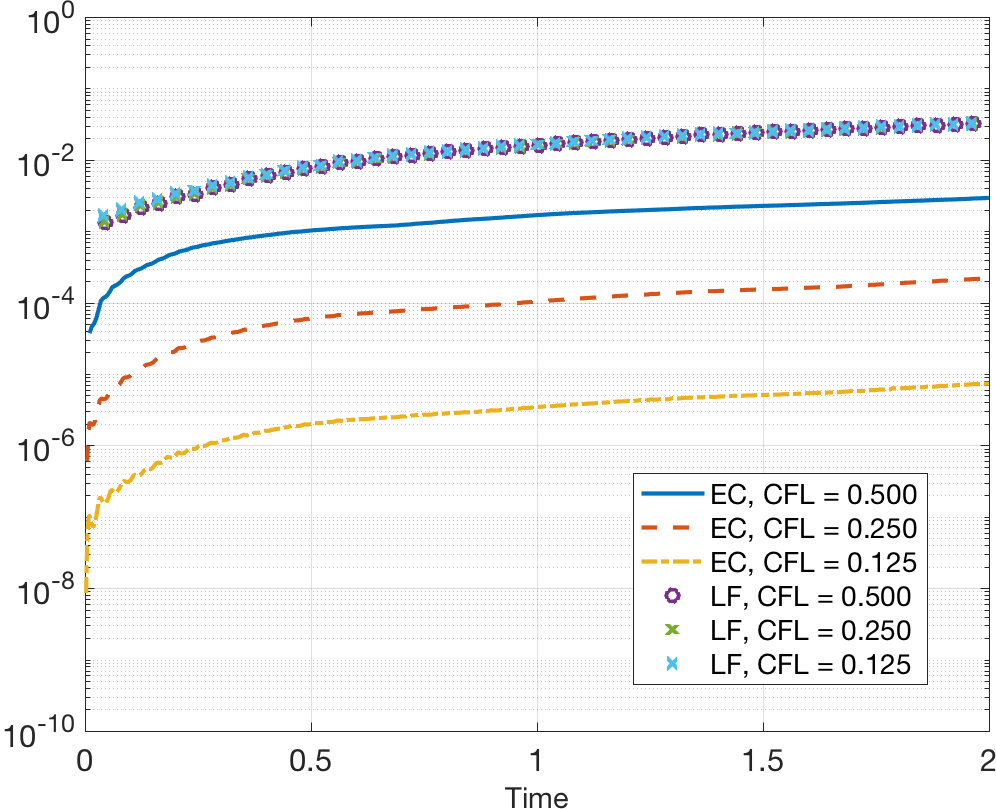
\includegraphics[width=.465\textwidth]{figs/dS_ECLF.png}}
\hspace{1em}
\subfloat[$\rho(x), u(x)$ ($N=4, K = 16$)]{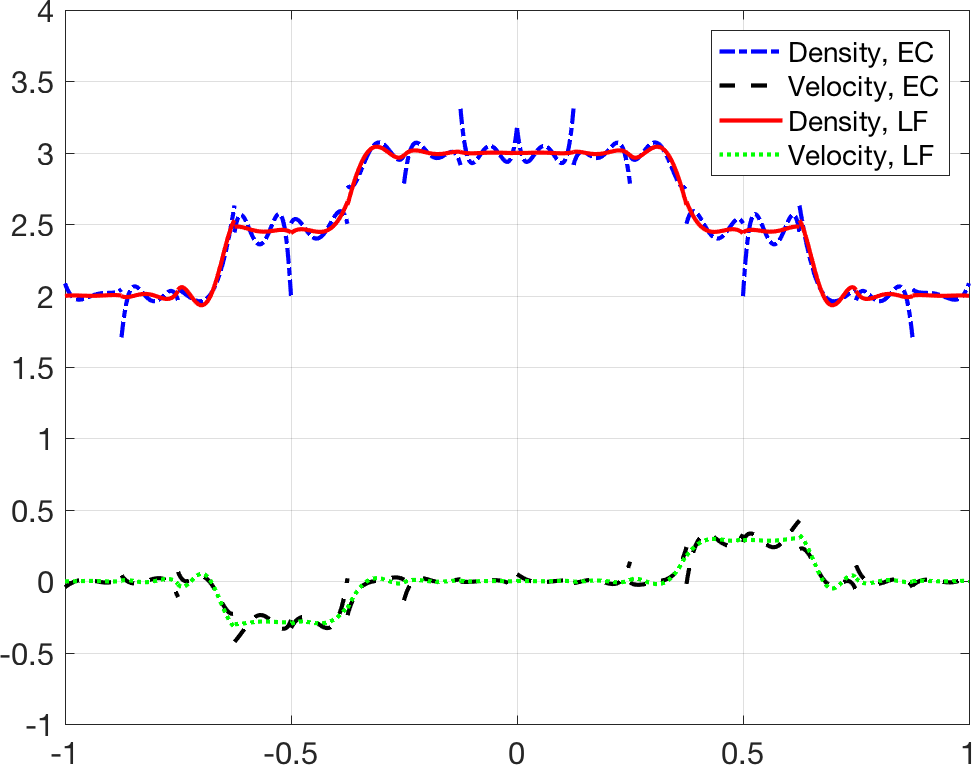
\includegraphics[width=.475\textwidth]{figs/sol_ECLF.png}}
\caption*{$\Delta S(\bm{u})$ and solution for entropy conservative (EC) and Lax-Friedrichs (LF) fluxes. }
\end{figure}

}

\frame{
\frametitle{Numerical experiments: Sod shock tube}

\begin{itemize}
\item Cell averages overlaid as circles.
\item CFL of .125 used for both GLL-$(N+1)$and GQ-$(N+2)$.
\end{itemize}
\begin{figure}
\centering
\only<1>{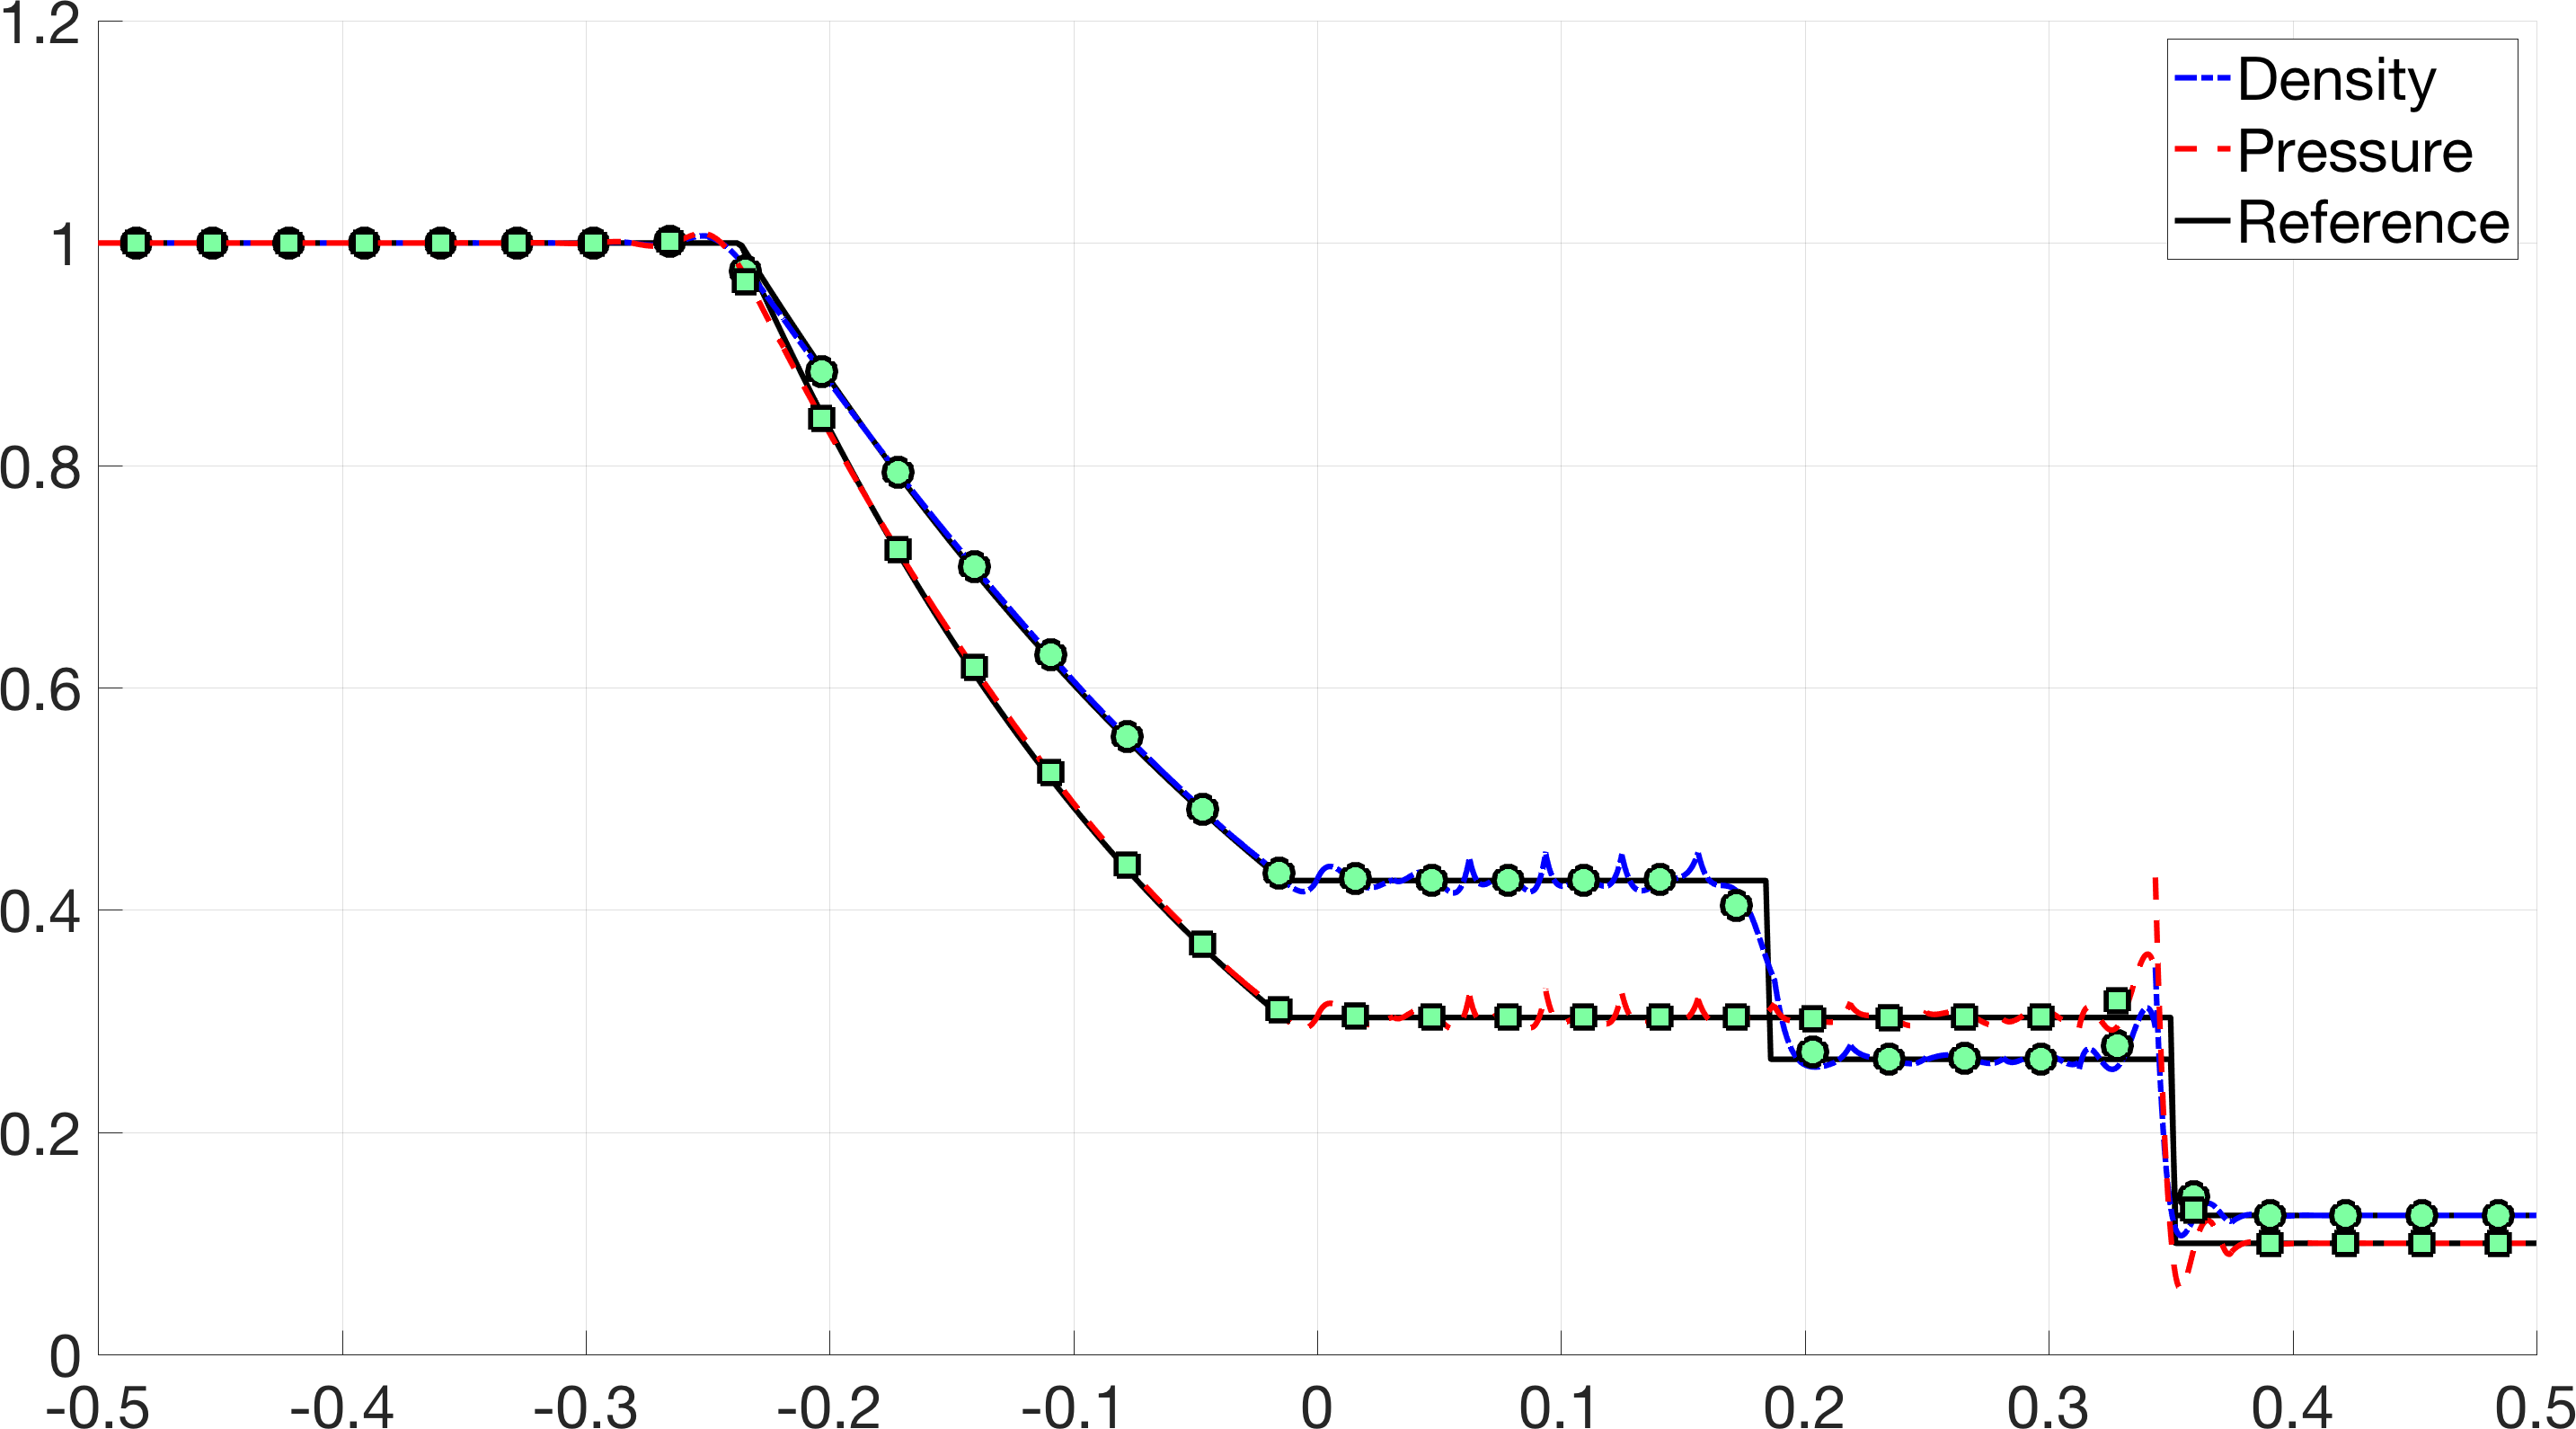
\includegraphics[width=.8\textwidth]{figs/sodGLL.png}\caption*{$N=4, K = 32$, $(N+1)$ point Gauss-Lobatto-Legendre quadrature.}}
\only<2>{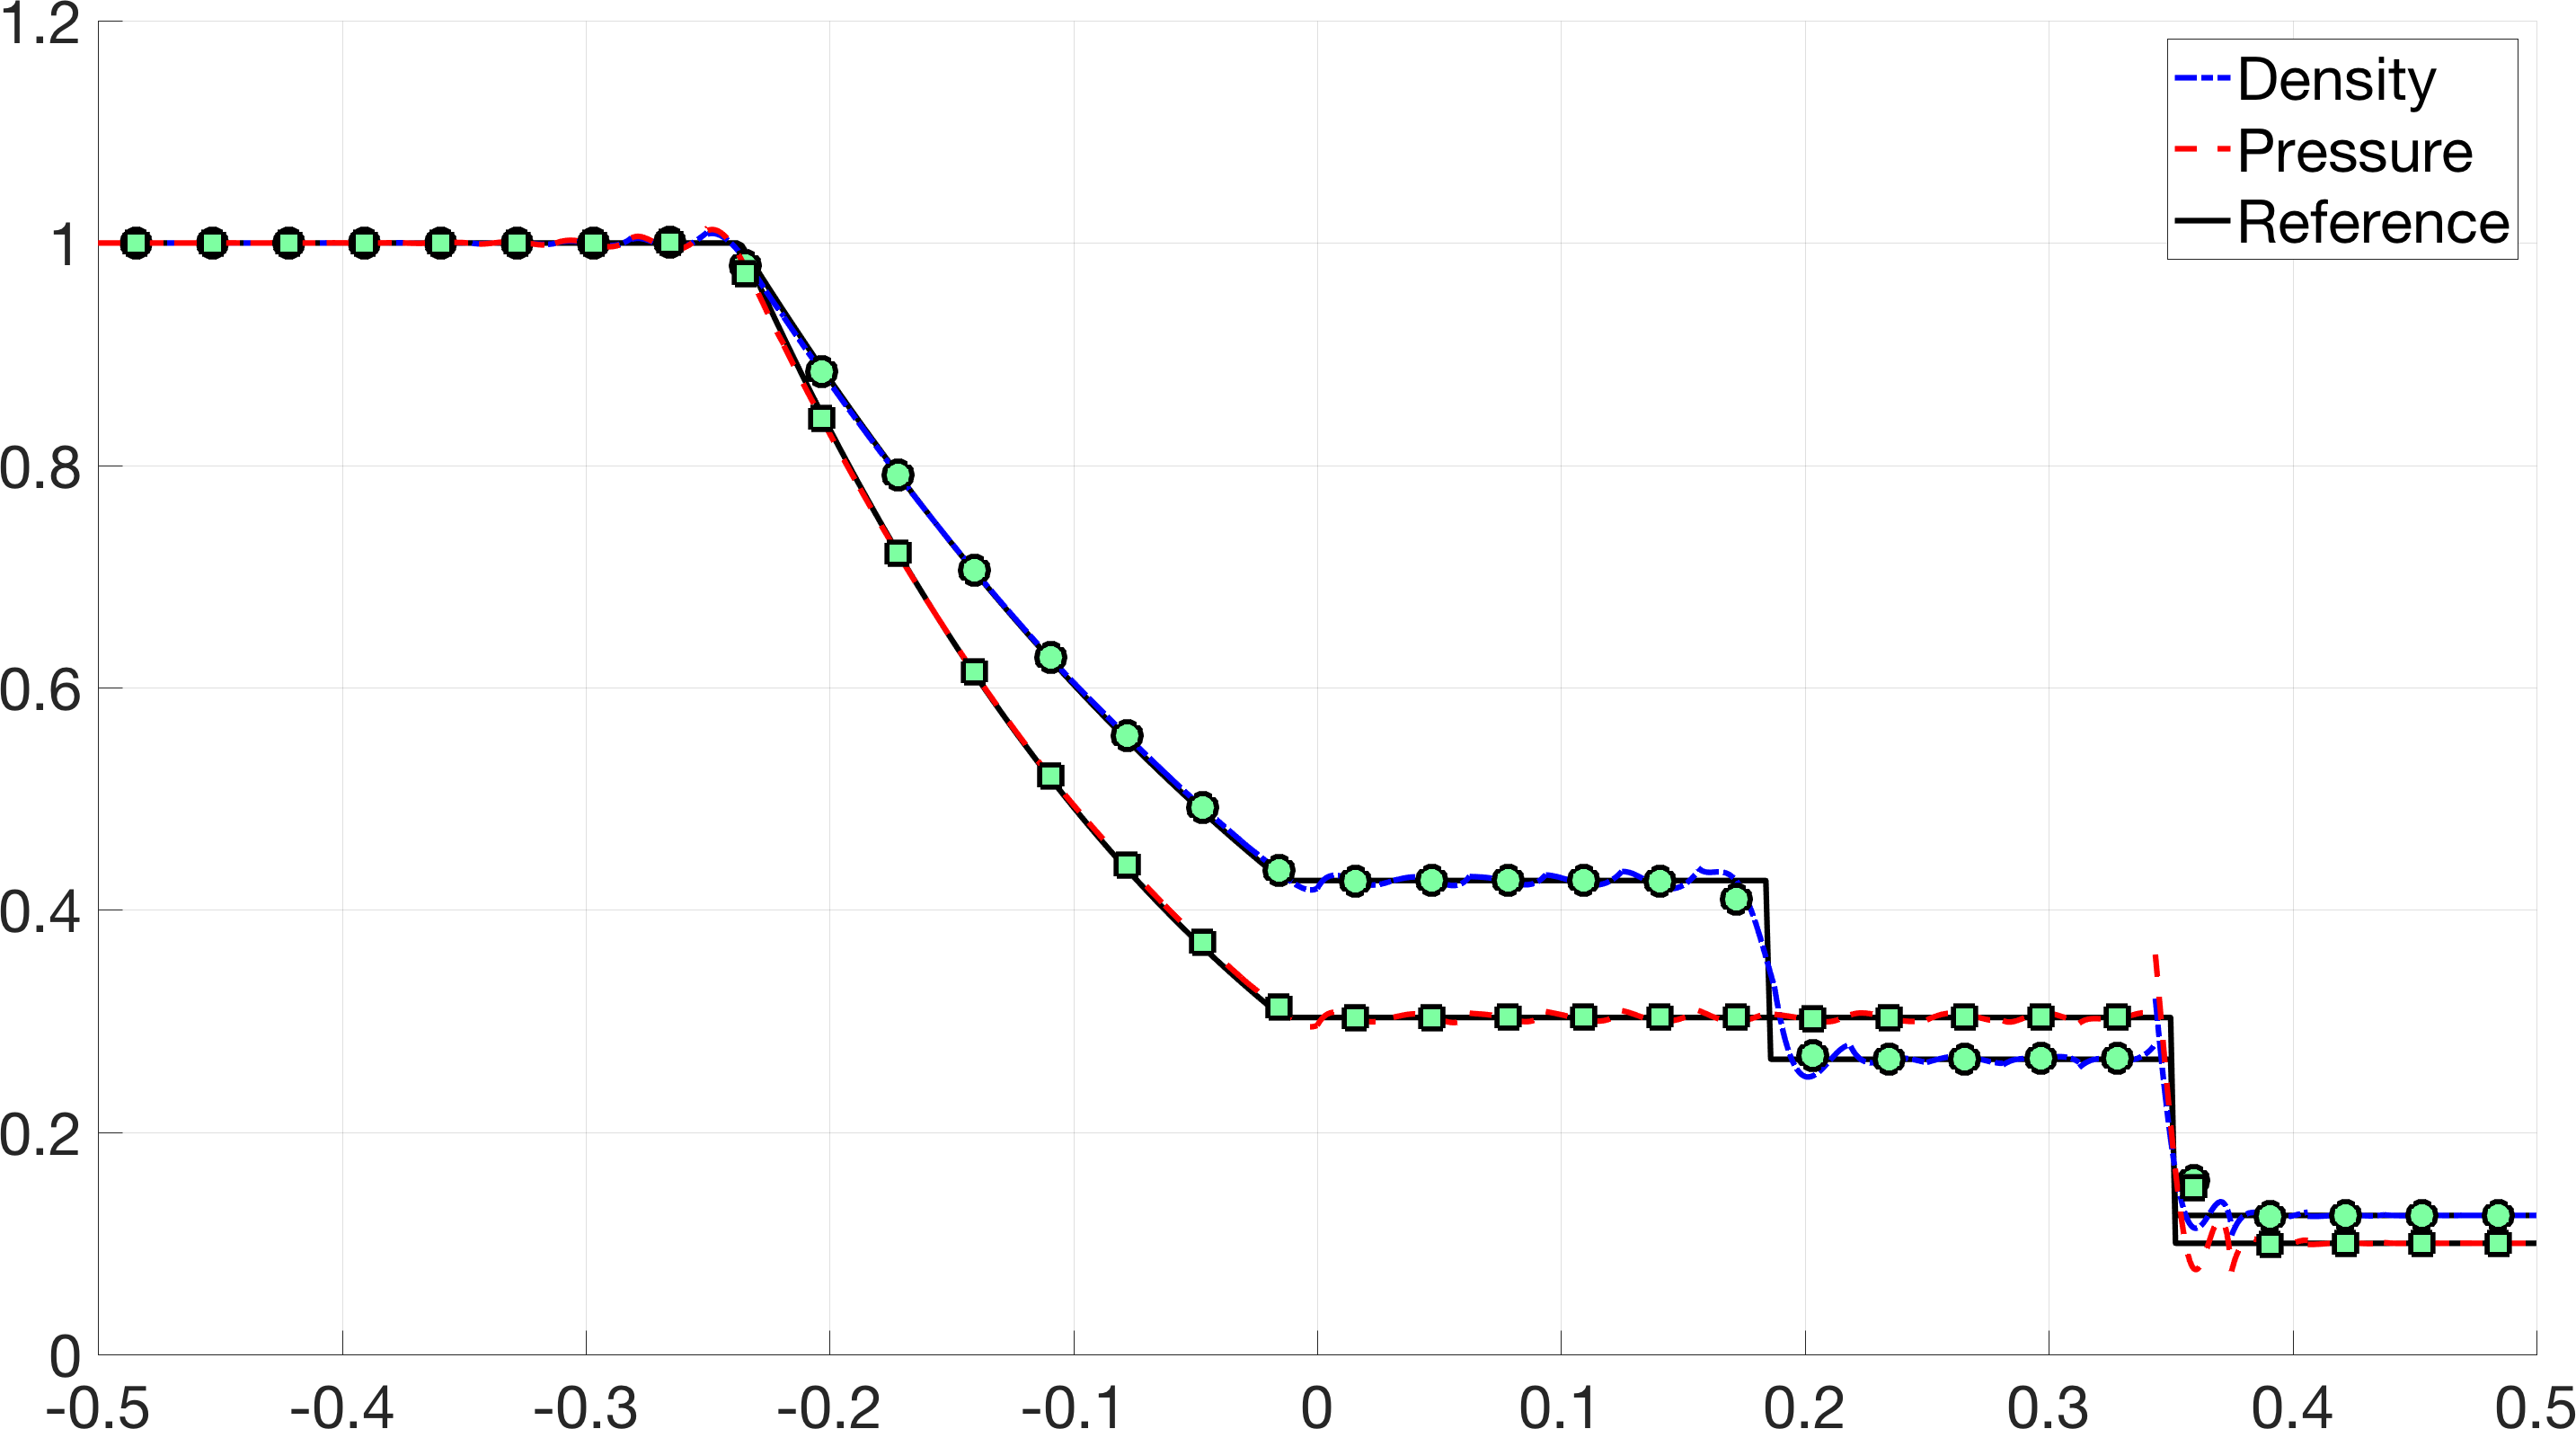
\includegraphics[width=.8\textwidth]{figs/sodGQ2.png}\caption*{$N=4, K = 32$, $(N+2)$ point Gaussian quadrature.}}
\end{figure}

}

\frame{
\frametitle{Numerical experiments: sine-shock interaction}

\begin{itemize}
\item Reference solution, smaller CFL (.05 vs .125) for GQ-$(N+2)$.  
\end{itemize}

\begin{figure}
\centering
\only<1>{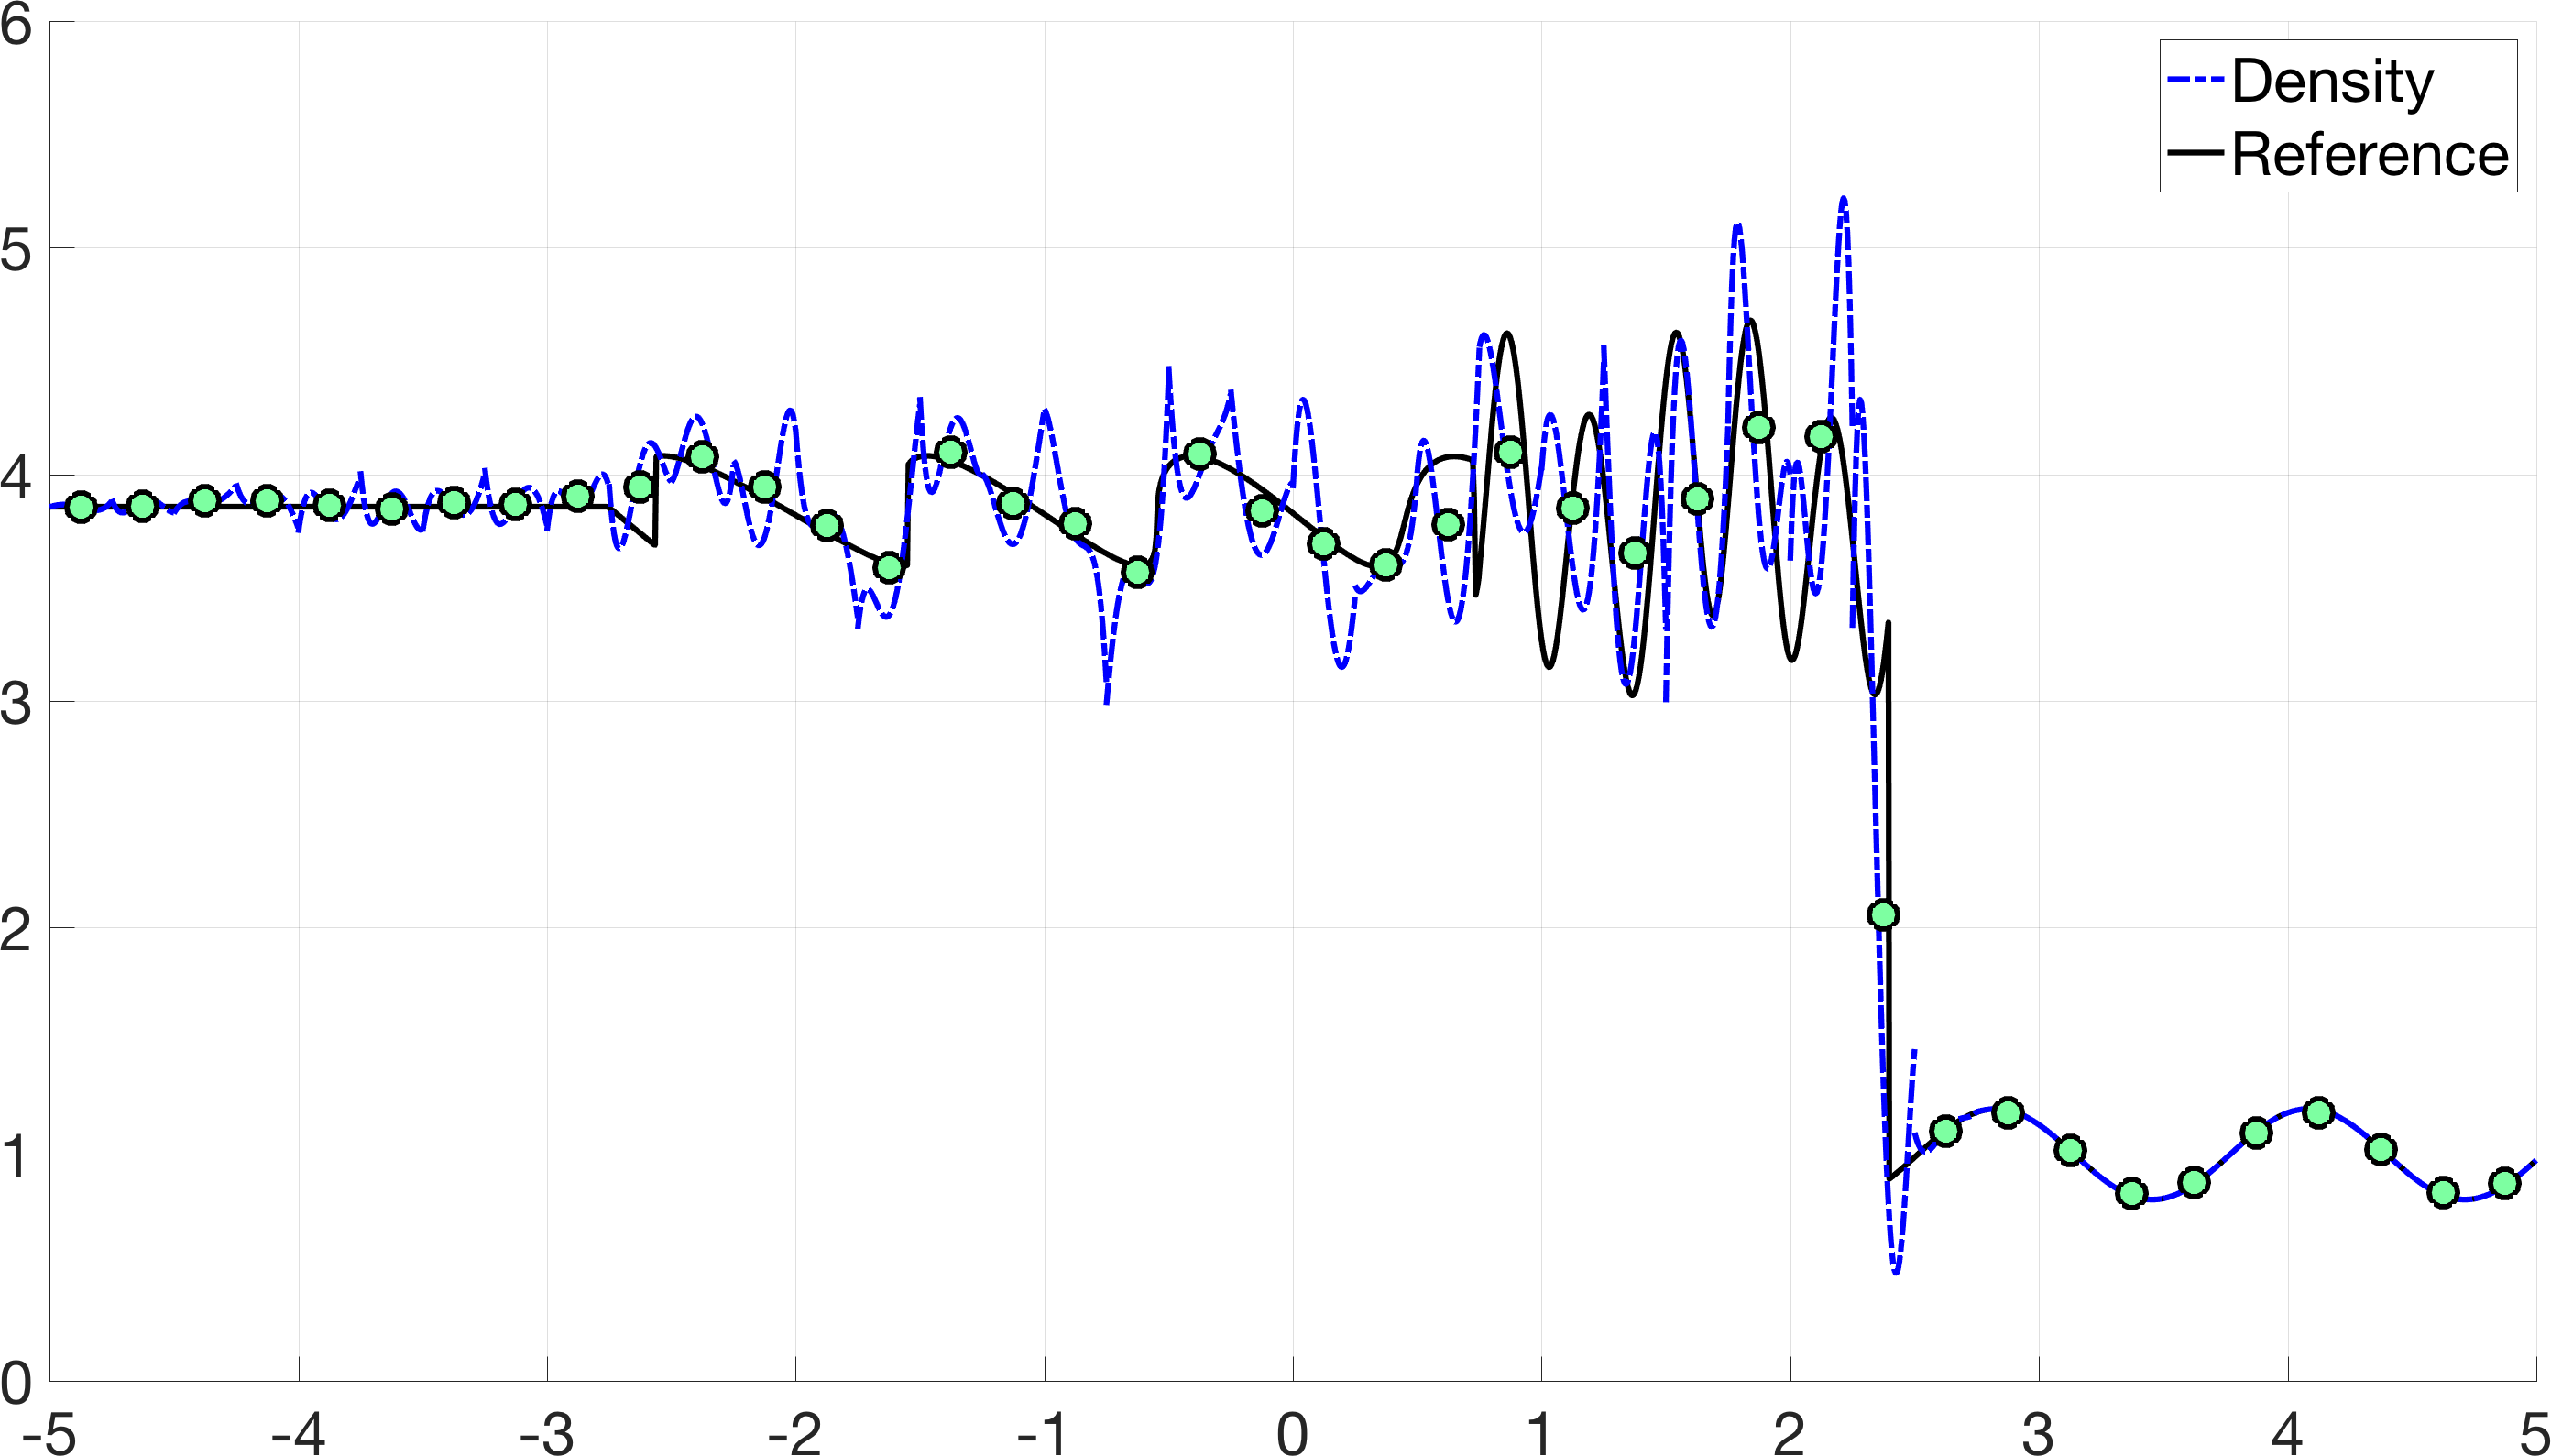
\includegraphics[width=.8\textwidth]{figs/sineShockGLL.png}\caption*{$N=4, K = 40$, $(N+1)$ point Gauss-Lobatto-Legendre quadrature.}}
\only<2>{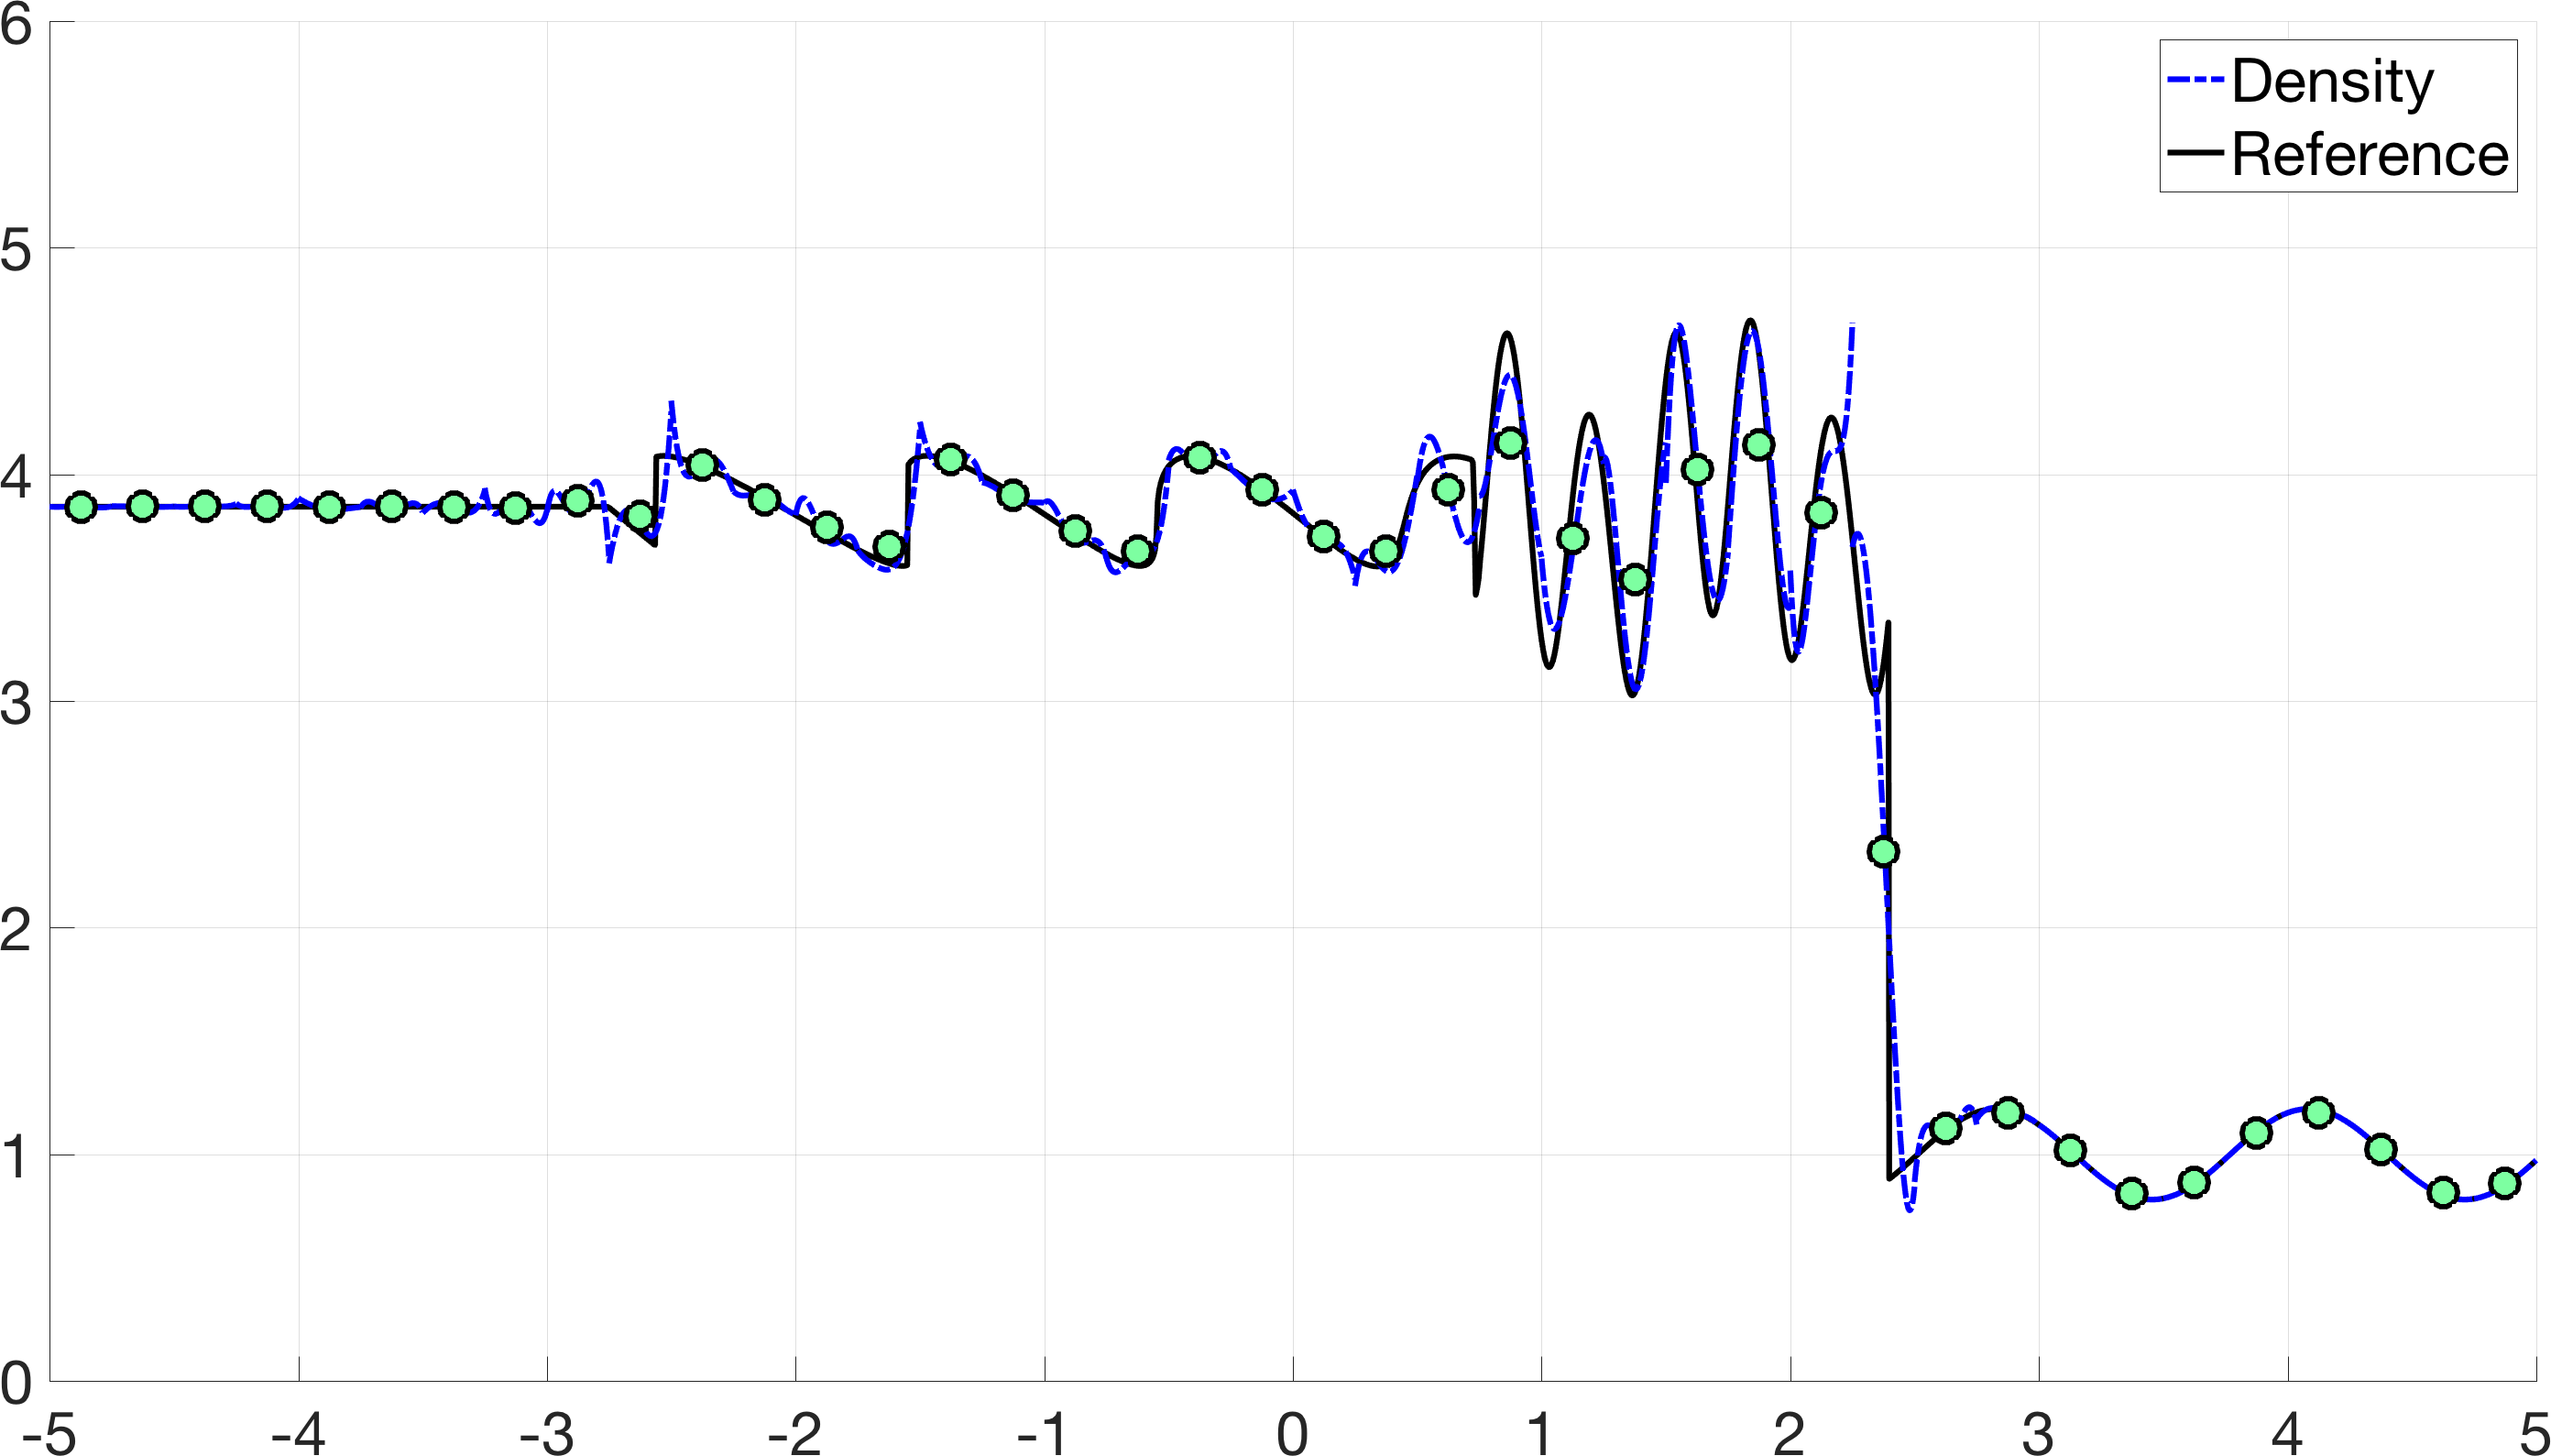
\includegraphics[width=.8\textwidth]{figs/sineShockGQ2.png}\caption*{$N=4, K = 40$, $(N+2)$ point Gaussian quadrature.}}
\end{figure}

}

\frame{
\frametitle{Numerical experiments: CFL restrictions}

\begin{itemize}
\item For GLL-$(N+1)$ quadrature, $\bm{u}\LRp{P_N \bm{v}} = \bm{u}$ at GLL points.
\item For GQ-$(N+2)$, discrepancy between $L^2$ projection and interpolation.
\item Still need \note{positivity} of thermodynamic quantities!
\end{itemize}
\vspace{-1em}
\begin{figure}
\centering
\subfloat[${v}_3(x), \LRp{P_N v_3}(x)$]{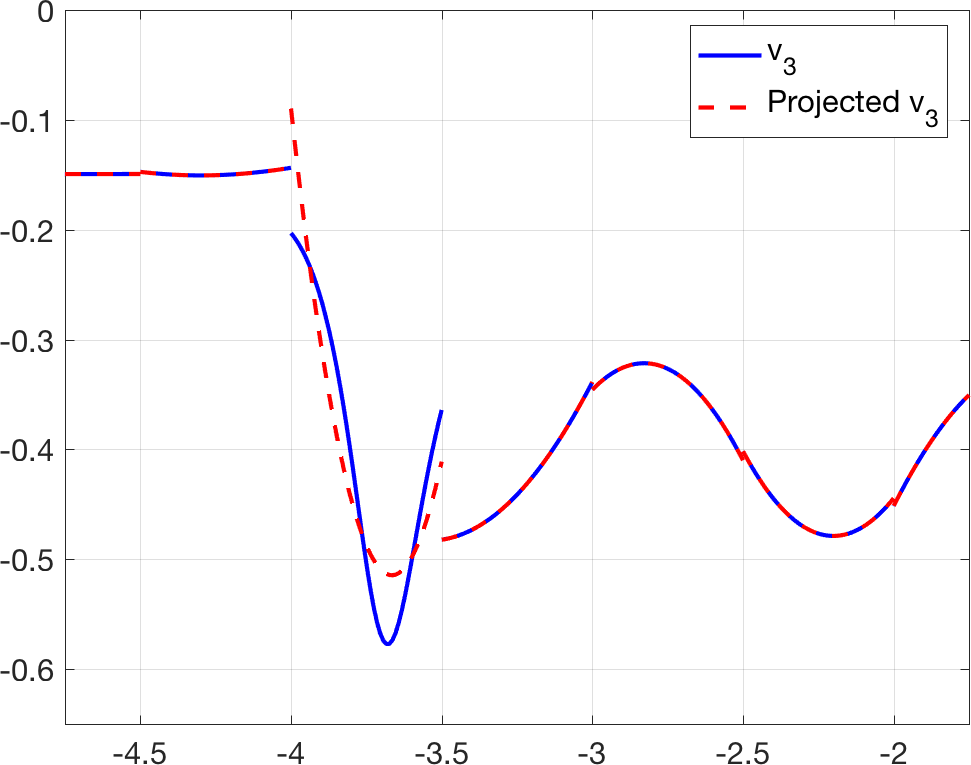
\includegraphics[width=.45\textwidth]{figs/sineShockQ3Compare.png}}
\hspace{1em}
\subfloat[$\rho(x), \rho\LRp{\LRp{P_N \bm{v}}(x)}$]{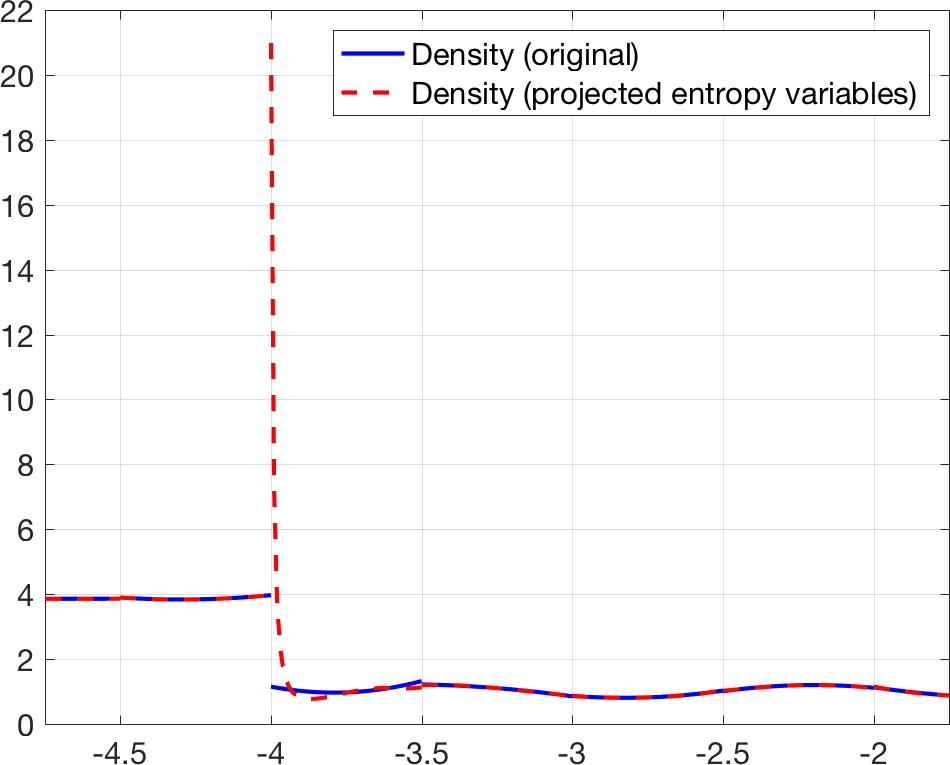
\includegraphics[width=.44\textwidth]{figs/sineShockDensityCompare.png}}
\end{figure}

}

\frame{
\frametitle{Extension to higher dimensions}

\begin{itemize}
\item Define global gradient, divergence, e.g.\
\begin{align*}
\LRp{\Grad_h\cdot\bm{u},v}_{\Omega} &= \sum_k \LRp{\Grad \cdot \bm{u}, v}_{D^k} + \LRa{\frac{1}{2}\jump{\bm{u}}\cdot\bm{n},v }_{\partial D^k}\\
\LRp{\Grad_h u,\bm{v}}_{\Omega} &= \sum_k \LRp{\Grad u, \bm{v}}_{D^k} + \LRa{\frac{1}{2}\jump{u}\bm{n},\bm{v}}_{\partial D^k}
\end{align*}
\item Flux differencing: let $\bm{u}_x = \bm{u}\LRp{P_N\bm{v}(\bm{x})}, \bm{u}_y = \bm{u}\LRp{P_N\bm{v}(\bm{y})}$
\[
\LRp{\pd{\bm{u}}{t} + \left.\LRp{2\Grad_h \cdot \bm{f}_S(\bm{u}_x,\bm{u}_y)}\right|_{\bm{y}=\bm{x}},\bm{w}}_{\Omega} = 0, \qquad \forall \bm{w}\in V_h.
\]
\item Entropy stability on curved meshes: modify flux using $\bm{G}_{ij} = \pd{\bm{x}_i}{\hat{\bm{x}}_j}$% $\Grad u = \bm{G}\hat{\Grad} u$, 
\[
\tilde{\bm{f}}_S(\bm{u}_L,\bm{u}_R) = \avg{J\bm{G}}\bm{f}_S(\bm{u}_L,\bm{u}_R).
\]
%\item Geometric mapping $\bm{x} = \bm{\Phi}\LRp{\hat{\bm{x}}}$ on $D^k$ and identities
%\begin{align*}
%&\bm{G}_{ij} = \pd{\bm{\Phi}_i}{\hat{\bm{x}}_j},& &J ={\rm det}\LRp{\hat{\Grad} \bm{\Phi}},& \\
%&\hat{\Grad}\cdot \LRp{J\bm{G}} = 0,& &\bm{n}J^f = J\bm{G}\hat{\bm{n}}.&
%\end{align*}
\end{itemize}

}

%\frame{
%\frametitle{Extension to curved meshes}
%
%\begin{itemize}
%\item Geometric mapping $\bm{x} = \bm{\Phi}\LRp{\hat{\bm{x}}}$ on $D^k$ and identities
%\begin{align*}
%&\bm{G}_{ij} = \pd{\bm{\Phi}_i}{\hat{\bm{x}}_j},& &J ={\rm det}\LRp{\hat{\Grad} \bm{\Phi}},& \\
%&\hat{\Grad}\cdot \LRp{J\bm{G}} = 0,& &\bm{n}J^f = J\bm{G}\hat{\bm{n}}.&
%\end{align*}
%\item New definitions of global DG gradient, divergence:
%\begin{align*}
%\LRp{\Grad_h \cdot \bm{u},v}_{\Omega} &= \sum_k \LRp{\hat{\Grad} \cdot P_N \LRp{ J\bm{G}^Tu} ,v}_{\hat{D}} + \LRp{\frac{1}{2}\LRp{J\bm{G}\hat{\bm{n}}}^T\jump{\bm{u}} ,v }_{\partial \hat{D}}\\
%\LRp{\Grad_h u,\bm{v}}_{\Omega} &= \sum_k \LRp{J\bm{G}\hat{\Grad} P_N u ,\bm{v}}_{\hat{D}} + \LRp{\frac{1}{2}J\bm{G}\bm{n} \jump{u} ,\bm{v}\cdot}_{\partial \hat{D}}
%\end{align*}
%\end{itemize}
%}

\frame{
\frametitle{ Numerical results: two-dimensional curvilinear meshes}
\setcounter{subfigure}{0}

\only<1>{
\begin{itemize}
\item Vortex problem at $T = 5$, $\Omega = [0,20]\times [-5,5]$, CFL = .25.  
\item Avoid weighted mass inverse using weight-adjusted approximation.
%\[
%\bm{M}_{J}^{-1} \approx \hat{\bm{M}}^{-1} \bm{M}_{1/J} \hat{\bm{M}}^{-1}.
%\]
\end{itemize}
\let\thefootnote\relax\footnotetext{\tiny Chan, Hewett, and Warburton (2016). \textit{Weight-adjusted discontinuous Galerkin methods: curvilinear meshes}.}
}
\only<2>{
$L^2$ error converges at $O(h^{N+1})$ up to time-stepper accuracy (LSERK-45).
}

\begin{figure}
\centering
\only<1>{
\subfloat[Uniform mesh]{
\includegraphics[width=.425\textwidth]{figs/vortexMeshUniform.png}}
\hspace{1em}
\subfloat[Warped mesh]{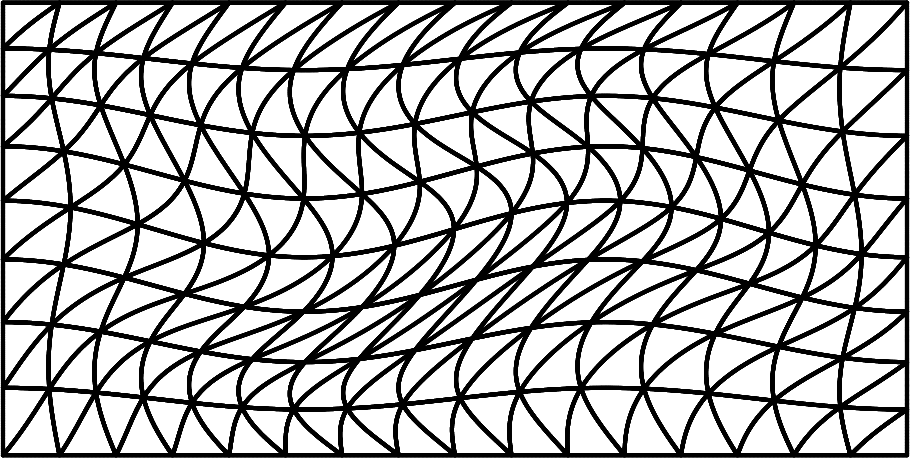
\includegraphics[width=.425\textwidth]{figs/vortexMeshCurved.png}}
}
\only<2>{
%\vspace{-1em}
\subfloat[Degree $N=1, N= 3$]{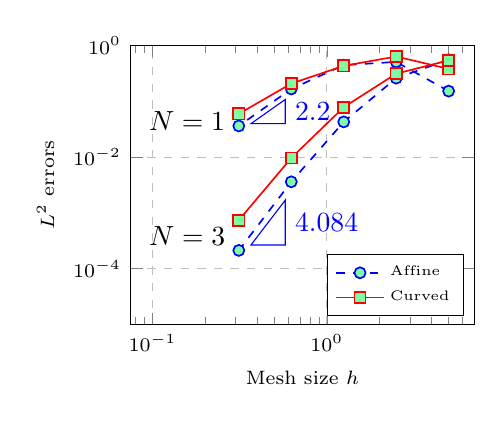
\begin{tikzpicture}
%\subfloat{\begin{tikzpicture}
\begin{loglogaxis}[
    width=.49\textwidth,
    xlabel={Mesh size $h$},  ylabel={$L^2$ errors}, 
    xmin=.075, xmax=7,
    ymin=1e-5, ymax=1,   
    legend pos = south east, legend cell align=left, legend style={font=\tiny},	
    xmajorgrids=true, ymajorgrids=true, grid style=dashed,
    legend entries={Affine, Curved}
] 
\pgfplotsset{
cycle list={{blue, dashed, mark=*}, {red, mark=square*}}
}
%\pgfplotsset{cycle list={{blue, dashed, mark=*}, {red, mark=square*}}}
\addplot+[semithick, mark options={solid, fill=markercolor}]
coordinates{(5,0.152443)(2.5,0.509207)(1.25,0.445656)(0.625,0.166519)(0.3125,0.036208)};
\addplot+[semithick, mark options={solid, fill=markercolor}]
coordinates{(5,0.380788)(2.5,0.636067)(1.25,0.432155)(0.625,0.207952)(0.3125,0.059728)}
[yshift=-2pt] node[left, pos=1.025, color=black] {$N = 1$};
\logLogSlopeTriangle{0.45}{0.1}{0.72}{2.2}{blue}

%\addplot+[semithick, mark options={solid, fill=markercolor}]
%coordinates{(5,0.484478)(2.5,0.46951)(1.25,0.125591)(0.625,0.015585)(0.3125,0.001791)};
%\addplot+[semithick, mark options={solid, fill=markercolor}]
%coordinates{(5,0.670522)(2.5,0.468234)(1.25,0.189765)(0.625,0.035238)(0.3125,0.005043)}
%[yshift=-1pt] node[left, pos=1.025, color=black] {$N = 2$};

\addplot+[semithick, mark options={solid, fill=markercolor}]
coordinates{(5,0.557086)(2.5,0.260022)(1.25,0.042815)(0.625,0.003611)(0.3125,0.000213)};
\addplot+[semithick, mark options={solid, fill=markercolor}]
coordinates{(5,0.54154)(2.5,0.312986)(1.25,0.07835)(0.625,0.00965)(0.3125,0.000739)}
[yshift=-4pt] node[left, pos=1.025, color=black] {$N = 3$};
\logLogSlopeTriangle{0.45}{0.1}{0.285}{4.084}{blue}

%\addplot+[semithick, mark options={solid, fill=markercolor}]
%coordinates{(5,0.463269)(2.5,0.169843)(1.25,0.017172)(0.625,0.000965)(0.3125,3.5e-05)};
%\addplot+[semithick, mark options={solid, fill=markercolor}]
%coordinates{(5,NaN)(2.5,0.247861)(1.25,0.043932)(0.625,0.002727)(0.3125,0.000118)}
%[yshift=1pt] node[left, pos=1.025, color=black] {$N = 4$};

\end{loglogaxis}
\end{tikzpicture}
}
%\hspace{1em}
\subfloat[Degree $N=2, N= 4$]{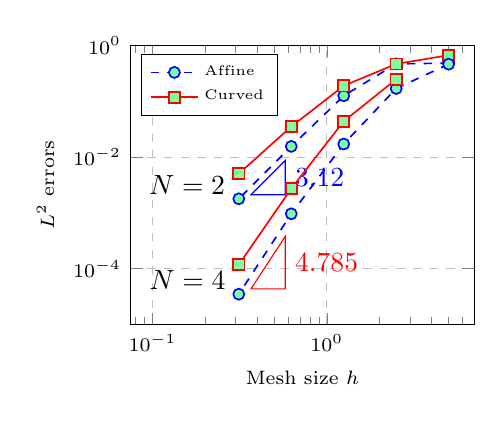
\begin{tikzpicture}
\begin{loglogaxis}[
    width=.49\textwidth,
    xlabel={Mesh size $h$},  ylabel={$L^2$ errors}, 
    xmin=.075, xmax=7,
    ymin=1e-5, ymax=1,
    legend pos = north west, legend cell align=left, legend style={font=\tiny},	
    xmajorgrids=true, ymajorgrids=true, grid style=dashed,
    legend entries={Affine, Curved}
] 
\pgfplotsset{
cycle list={{blue, dashed, mark=*}, {red, mark=square*}}
}
%\addplot+[semithick, mark options={solid, fill=markercolor}]
%coordinates{(5,0.152443)(2.5,0.509207)(1.25,0.445656)(0.625,0.166519)(0.3125,0.036208)};
%\addplot+[semithick, mark options={solid, fill=markercolor}]
%coordinates{(5,0.380788)(2.5,0.636067)(1.25,0.432155)(0.625,0.207952)(0.3125,0.059728)}
%[yshift=-2pt] node[left, pos=1.025, color=black] {$N = 1$};
%\logLogSlopeTriangle{0.45}{0.05}{0.625}{2.2}{blue}

\addplot+[semithick, mark options={solid, fill=markercolor}]
coordinates{(5,0.484478)(2.5,0.46951)(1.25,0.125591)(0.625,0.015585)(0.3125,0.001791)};
\addplot+[semithick, mark options={solid, fill=markercolor}]
coordinates{(5,0.670522)(2.5,0.468234)(1.25,0.189765)(0.625,0.035238)(0.3125,0.005043)}
[yshift=-3pt] node[left, pos=1.025, color=black] {$N = 2$};
\logLogSlopeTriangle{0.45}{0.1}{0.465}{3.12}{blue}

%\addplot+[semithick, mark options={solid, fill=markercolor}]
%coordinates{(5,0.557086)(2.5,0.260022)(1.25,0.042815)(0.625,0.003611)(0.3125,0.000213)};
%\addplot+[semithick, mark options={solid, fill=markercolor}]
%coordinates{(5,0.54154)(2.5,0.312986)(1.25,0.07835)(0.625,0.00965)(0.3125,0.000739)}
%[yshift=-4pt] node[left, pos=1.025, color=black] {$N = 3$};
%\logLogSlopeTriangle{0.45}{0.05}{0.075}{4.084}{blue}

\addplot+[semithick, mark options={solid, fill=markercolor}]
coordinates{(5,0.463269)(2.5,0.169843)(1.25,0.017172)(0.625,0.000965)(0.3125,3.5e-05)};
\addplot+[semithick, mark options={solid, fill=markercolor}]
coordinates{(5,NaN)(2.5,0.247861)(1.25,0.043932)(0.625,0.002727)(0.3125,0.000118)}
[yshift=-4pt] node[left, pos=1.025, color=black] {$N = 4$};
\logLogSlopeTriangle{0.45}{0.1}{0.1275}{4.785}{red}
\end{loglogaxis}
\end{tikzpicture}
}
}

\end{figure}
}


%% =================================================

\frame{
\frametitle{Summary and acknowledgements}

\begin{itemize}
\item Derived discretely entropy stable high order discontinuous Galerkin methods using a continuous formulation.  
\vspace{.5em}
\item Future work: regularization, multi-GPU (with Lucas Wilcox).
\vspace{.5em}
\item This research is supported by the National Science Foundation under awards DMS-1712639 and DMS-1719818. 
\end{itemize}
\vspace{.5em}
\begin{center}
Thank you!  Questions?
\vspace{1em}

{
\includegraphics[width=.15\textwidth]{figs/nsf.jpg}}
\end{center}


\let\thefootnote\relax\footnotetext{\tiny Chan, Hewett, and Warburton (2016). \textit{Weight-adjusted discontinuous Galerkin methods: curvilinear meshes}.}
\let\thefootnote\relax\footnotetext{\tiny Chan (2017). \textit{On discretely entropy conservative and entropy stable discontinuous Galerkin methods.}}

}

%% =================================================


\begin{frame}[noframenumbering]
\frametitle{Additional slides }
\end{frame}


\frame[noframenumbering]{
\frametitle{Global DG differentiation operator}
\vspace{-.5em}
\begin{itemize}
\item Let $v\in V_h$, $u, w\not\in V_h$ with $u,w$ bounded; modified $D^x_h$
\begin{align*}
\LRp{D^x_h u, vw}_{\Omega} &= \sum_k \LRp{\pd{P_N u}{x},vw}_{D^k} \\
& + \frac{1}{2} \LRa{u^+ - P_N u,vw\bm{n}_x}_{\partial D^k} \\
&+ \frac{1}{2} \LRa{u - P_N u,P_N\LRp{vw}\bm{n}_x}_{\partial D^k}.
\end{align*}
\item Integration-by-parts property
\[
\LRp{D^x_h u, vw}_{\Omega} = \LRa{u,vw}_{\partial \Omega} - \LRp{ u, D^x_h\LRp{vw}}_{\Omega}.
\]
\item Coupling only through \note{surface} values (in contrast to $D^x_h$ with $\jump{P_N u}$).
\end{itemize}
\let\thefootnote\relax\footnotetext{\tiny Chen and Shu (2017). \textit{ES high order DG methods with suitable quadrature rules for hyperbolic conservation laws.}}
}

\bibliographystyle{plain}
{\scriptsize
\bibliography{pyramids}
}

\end{document}
